% !TEX encoding = UTF-8
% !TEX TS-program = pdflatex
% !TEX root = ../Tesi.tex
% !TEX spellcheck = en-EN

%************************************************
\chapter{Numerical Simulation}
\label{cap:numericalsimulation}
%************************************************

\citet{RefWorks:172} define a \acs{DEM} numerical simulation as a computational
approximation of a real particulate material, represented as an ensemble of discrete, or distinct, elements, which
interact among each other according to defined contact laws.
Thus, under given hypotheses, we could use this simulation method to investigate
the nature and the behaviour of any granular medium.\\

\section{Software}
\label{sec:software}

We used the public open source \acs{DEM} software \acs{LIGGGHTS} as simulation toolbox.
\citet{RefWorks:136, RefWorks:206} demonstrated its effectiveness.
Especially, it is an highly parallelized software, which allowed us to perform
our simulations on large scale clusters.\\
Performing a simulation with \acs{LIGGGHTS} consists of two steps:
\begin{enumerate}
  \item{write a script, stating the involved domain, the chosen contact laws,
  and the microscopic parameters of these laws;}
  \item{running the script in bash with single or multiple cores.}
\end{enumerate}

\section{Microscopic parameters}
\label{sec:microscopicparameters}

In our work, we decided to utilize a single
contact law for all the simulations performed (see \citet{RefWorks:205}).\\
Following the indications summarized in Section \ref{sec:timestep}, we chose
time steps between $1.29 \%$ and $1.53 \%$ of the Rayleigh time, 
depending on the particle density (\acs{rhop}) and on the particle size.
Furthermore, we kept constant the size distribution, which was obtained by
experimental sieving, see Table \ref{tab:19particlesizedistributions}.\\
The \acs{DEM} values for the Young's modulus (\acs{E}) and the Poisson's
coefficient (\acs{nu}) were taken from the literature and kept identical for
each simulation, see \cite{RefWorks:175} and \cite{RefWorks:176}. However, we
reduced the former to increase the time step (\acs{deltat}), following the recommendations of Ai et al.
\cite{RefWorks:131}.
The values can be found in Table \ref{tab:09DEMFixedinputvalues}. \\

\begin{table}[h]
\centering
\begin{tabular}{ccc}
\hline
    Young's & Poisson's & \acs{deltat}\\
   modulus & ratio & \\
    $[MPa]$ & $[-]$ & [s]\\
    \hline
    $10$    & $0.40$ & $10^{-6}$\\


\hline
\end{tabular}
\caption{DEM fixed input values}
\label{tab:09DEMFixedinputvalues}
\end{table}

\section{Macroscopic parameters}
\label{sec:macroscopicparameters}

A Matlab script allowed us to extract from the simulation output the numerical
values representative of bulk behaviour (hereafter called \textit{bulk values}),
see Table \ref{tab:14bulkvalues},
for each \acs{DEM} simulation parameter combination.

\section{Drained Angle of Repose Simulation}
\label{sec:aorsim}

In \acs{AoR} simulations we sought to replicate meticulously the experimental
setup explained in Section \ref{sec:aor}, considering both the plate and the
liftable boundary, with the same domain size consideration as before see Fig. \ref{fig:065aorsim}. 
The particles had the same properties as in the shear-cell simulation. 
The first phase was identical to that of the shear-cell simulation. 
After lifting the boundary, the particles formed a heap.
An image post-processing software was used to obtain the average slope.
In the \acs{AoR} tests the average of the repose angles provided us with the fourth
bulk value of Table \ref{tab:14bulkvalues}.
\begin{figure}[!htb]
\centering
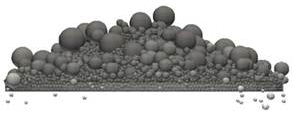
\includegraphics[width=.50\columnwidth]{images/065aorsim}
\caption[AoR sim]{Angle of repose simulation.}
\label{fig:065aorsim}
\end{figure}

\section{Shear Cell Simulation}
\label{sec:scsimulation}
%************************************************

\begin{figure}[!htb]
\centering
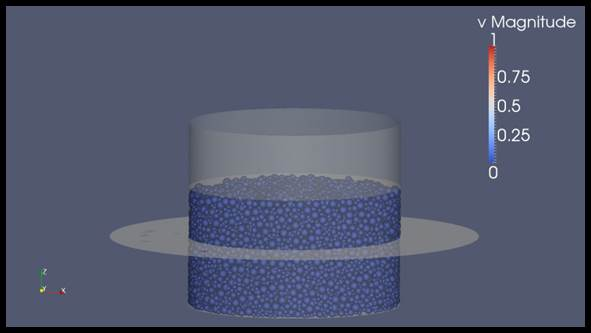
\includegraphics[width=.80\columnwidth]{images/007shearcellsim}
\caption[Shear cell simulation]{Shear cell simulation. The experimental device
was meticolously reproduced.}
\label{fig:007shearcellsim}
\end{figure}
\acs{LIGGGHTS}, the simulation toolbox we used, meets all the requirements of
modelling the shear tester described in Section \ref{sec:jsct}. 
First, it is capable of importing triangulated meshes of the two rings and a top lid. 
Since the real setup had a wall thickness, contact forces acting on a mesh are summed and can be saved, 
and thus shear force calculation is available out of the box. 
Second, the code can move a mesh with constant 
velocity as required for the measurement. 
To determine the shear stresses, the bulk solid had to be stressed with 
user-defined normal stresses. 
Therefore, a stress-controlled wall (servo-wall in \acs{LIGGGHTS}) was applied to the lid. \\
Although the geometry differs, the \acs{SCT} was designed to obtain the same values for the shear stresses as the 
Jenike shear cell tester (\acs{JSCT}), but with improved automation and reliability,
see Schulze \cite{RefWorks:118}. 
For this reason, the simulation setup was
based on the \acs{JSCT}, see Fig. \ref{fig:007shearcellsim}.
As suggested by Aigner et al. \cite{RefWorks:139} and Benvenuti et al. \cite{RefWorks:173}, 
the diameter and the height of the rings operated in the simulations had to be sufficiently large to avoid relevant wall effects. 
However, a larger domain increases the number of particles and thus
simulation time.
For this reason, we considered the cylinder dimension (\acs{dCylDp}), which is
proportional to the mean particle diameter, as an additional \acs{DEM}
parameter to be investigated.

\subsection{SCT simulation procedure}
\label{subsec:scsimulation}

A simulation run comprised four phases. 
First, the shear cell was filled with the granulate material, and it was allowed
to settle.
Then, the top lid was lowered and the first normal stress applied to the bulk
solid.
As in the experiment, the servo-wall allows calculating the position of the lid
while the first particle is being touched. 
The distance between the lid and the bottom of the domain multiplied by the 
simulation area gave the total volume.
Since the software already provided the total mass, we were able to calculate
the bulk density (\acs{rhob}).\\
Next, the ring moved by a distance $l=0.1875 \cdot radius ~of ~the ~ring$, and
the required pre-shear force was measured.
Finally, the normal load was reduced to a fraction of the initial load, 
the ring was moved again by a distance $l$, and the shear force was recorded. 
Unlike in the original experiment, the bottom ring was moved to facilitate the numerical simulation. 
The velocity of the ring displacement, and consequently the total simulation time, 
was determined by a trade-off between minimizing the normal load oscillation and
optimizing computation time. 
The former requires (relatively) low velocity, and the latter requires high
speed.
We chose a constant velocity of $3*(mean ~ particle ~ radius)/seconds$, as the
best trade-off.\\
The normal stresses (pre-shear and shear phases) applied in each simulation were
the same as in the experiments.
The corresponding $\tau_{psh}$ and $\tau_{sh}$ were calculated - as in the experiments - from the mean of the plateau.\\

\subsection{SCT Simulation Input Parameters}
\label{subsec:sctsimulationinputparameters}

The input \acs{DEM} coefficients, \acs{CoR}, \acs{mus}, \acs{mur},
\acs{rhop} and \acs{dCylDp} (the cylinder dimension, proportional to the mean
particle diameter), as indicated in Table \ref{tab:10DEMVariableinputvalues}, 
were constant in each simulation, but their combination differed between
simulations.
Further, \acs{dCylDp} was used to evaluate the wall effect, but only $~10\%$ of the
simulations had a \acs{dCylDp} larger than $20$.
The normal stress \acs{sigman} and its
percentage during the incipient flow condition \acs{tauperc}
varied to replicate twelve shear-cell load conditions.\\ 

\subsection{SCT Simulation Output Parameters}
\label{subsec:sctsimulationoutputparameters}

\begin{figure}[!htb] 
\centering 
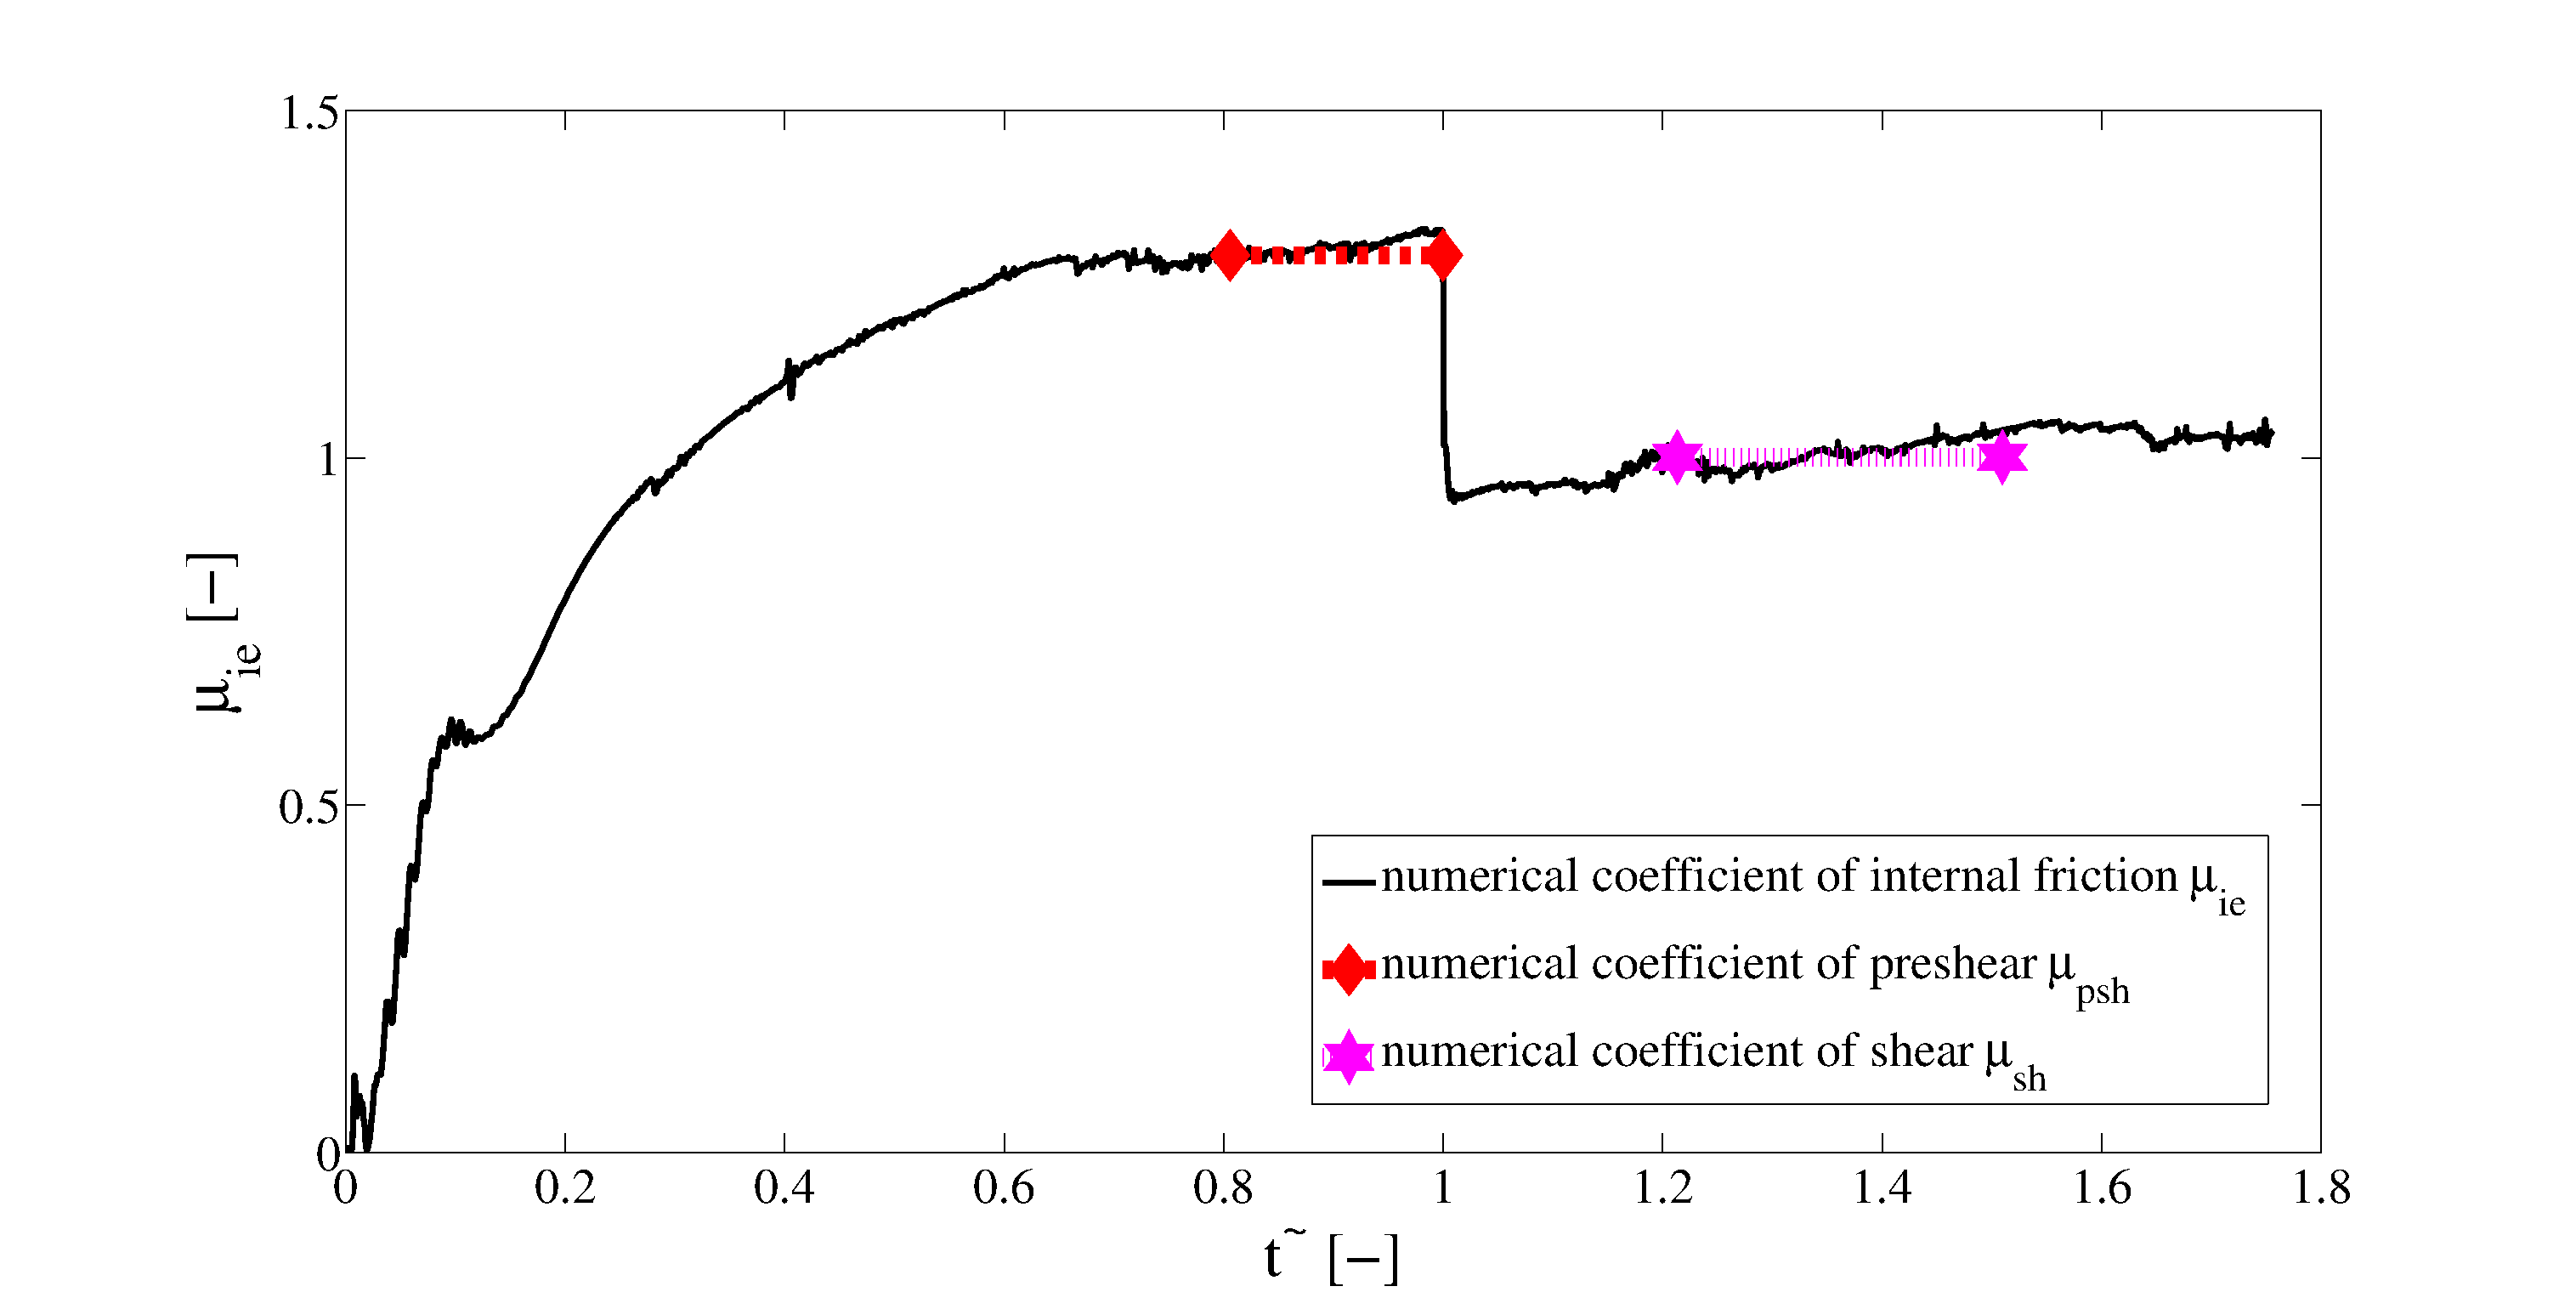
\includegraphics[width=.96\textwidth]{images/021simexample} 
\caption[Numerical shear cell tester stress path]{Numerical shear-cell tester
stress path - $\sigma_n = 10000 ~Pa$.}
\label{fig:021simexample} 
\end{figure}

% \begin{figure}[htp] \centering
%     \begin{subfigure}[b]{0.96\columnwidth}
%         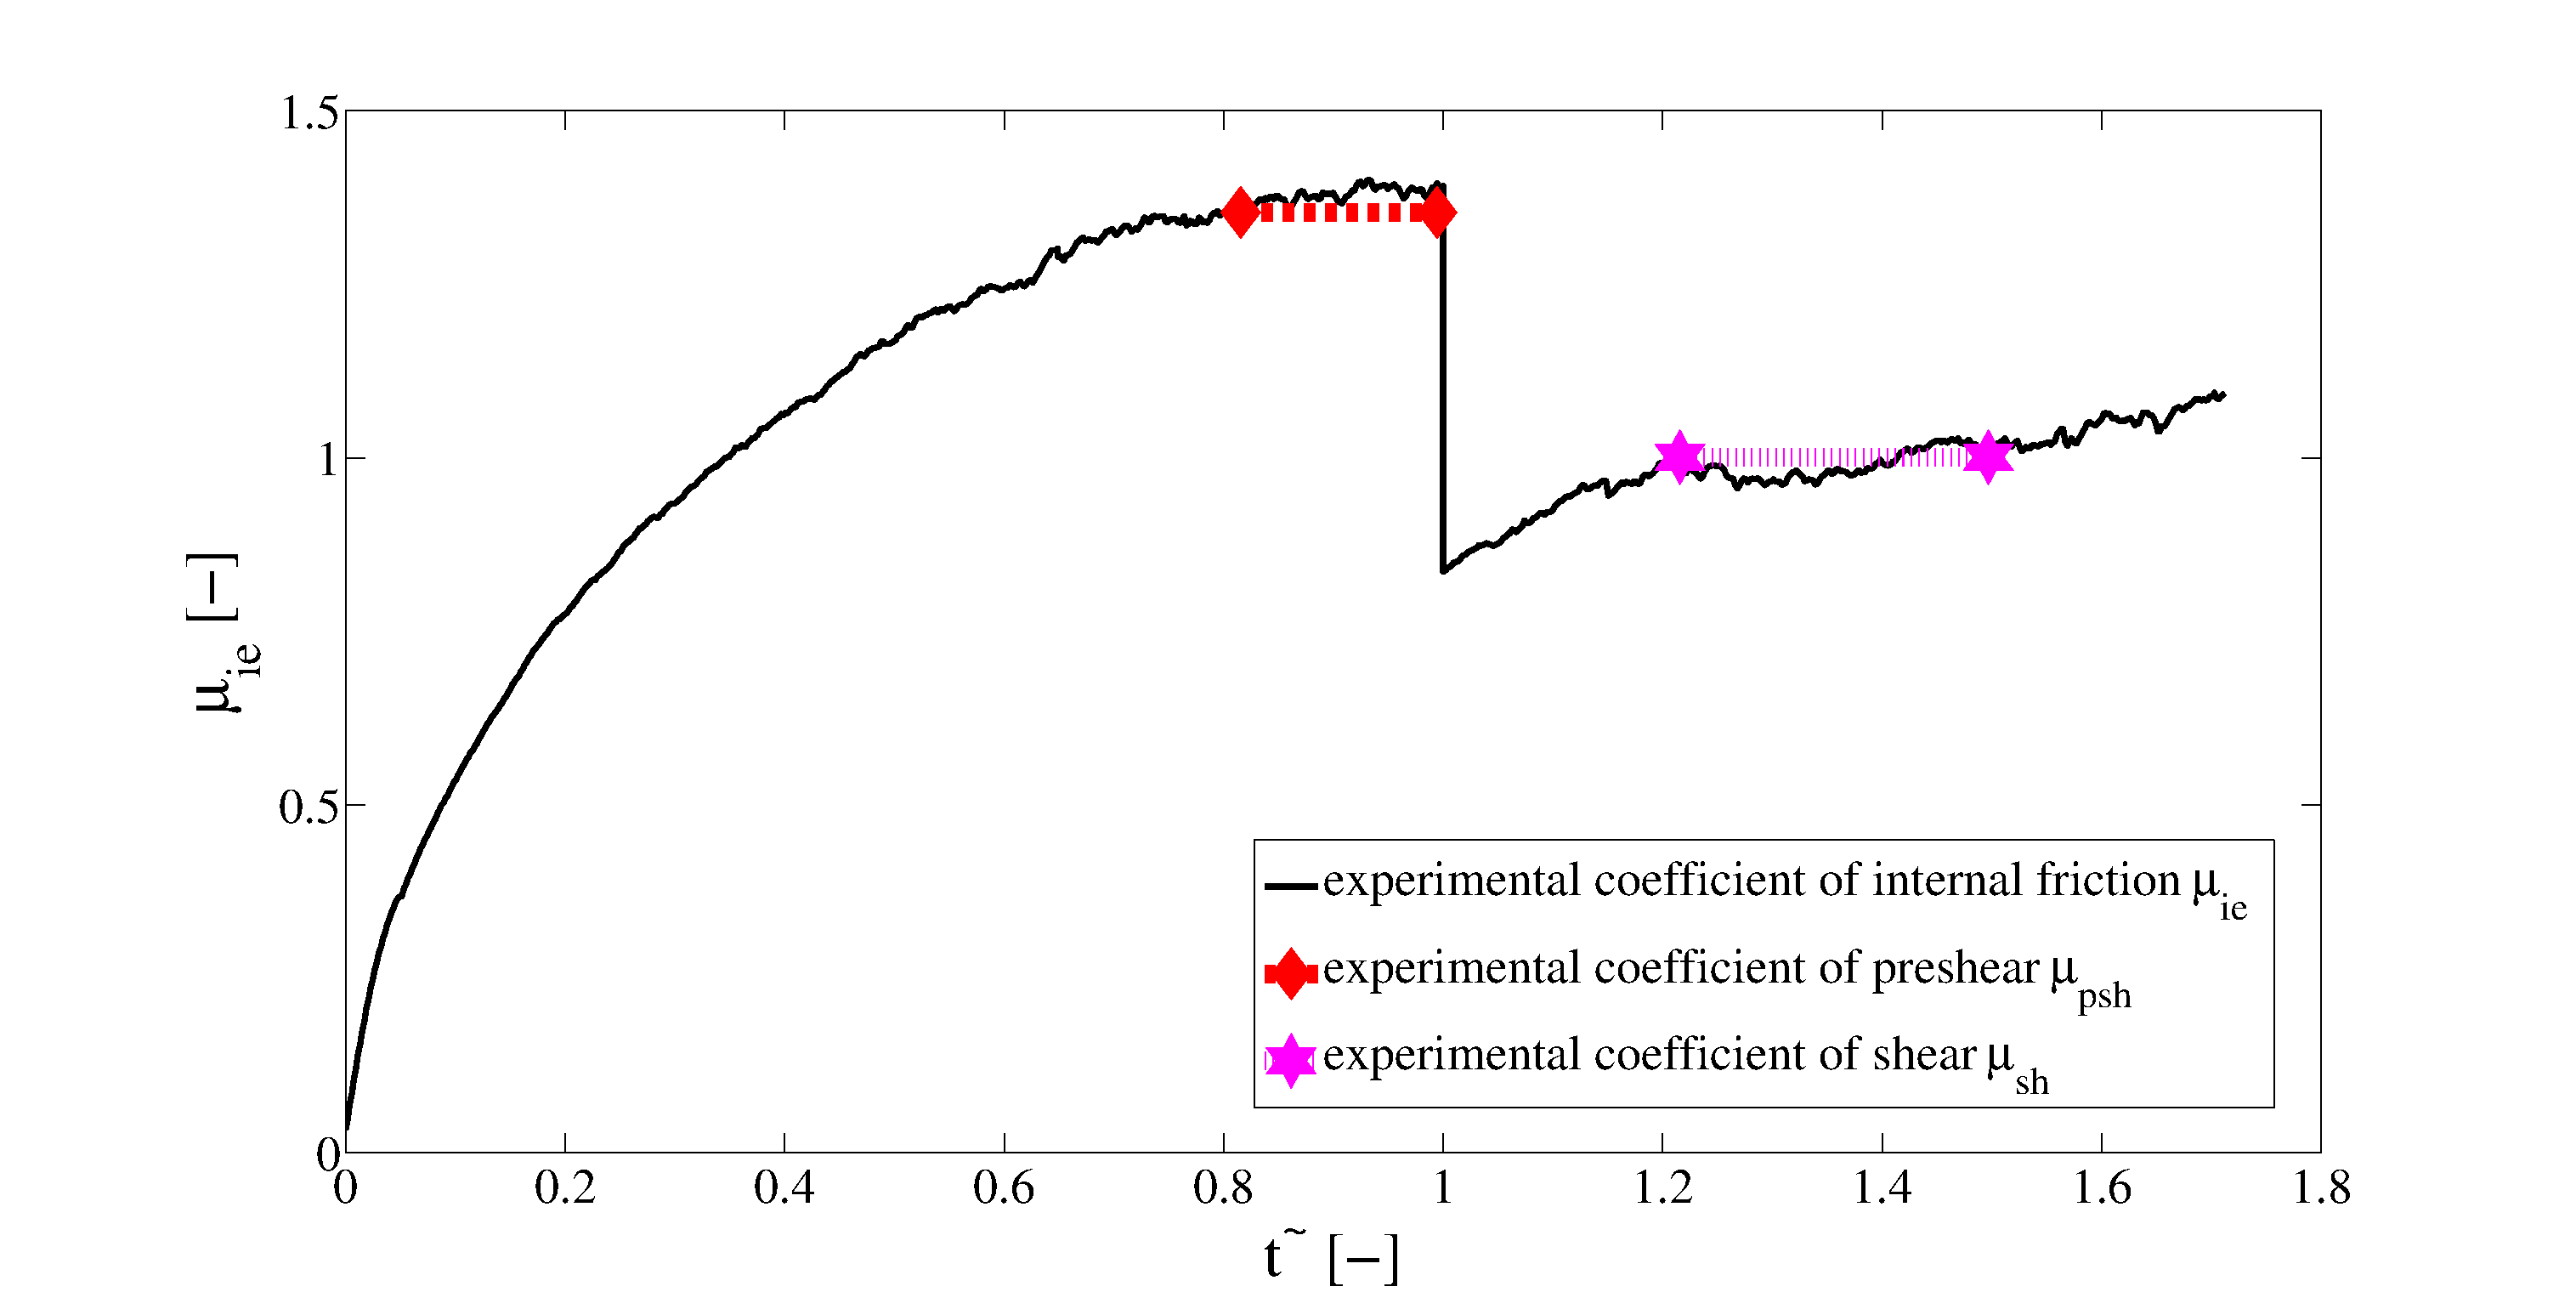
\includegraphics[width=\textwidth]{20experimental}
%         \caption{Experimental shear-cell tester stress path - $\sigma_n = 10000
%         ~Pa$}
%         \label{fig:20experimental} 
%     \end{subfigure}\\
%         \begin{subfigure}[b]{0.96\columnwidth}
%         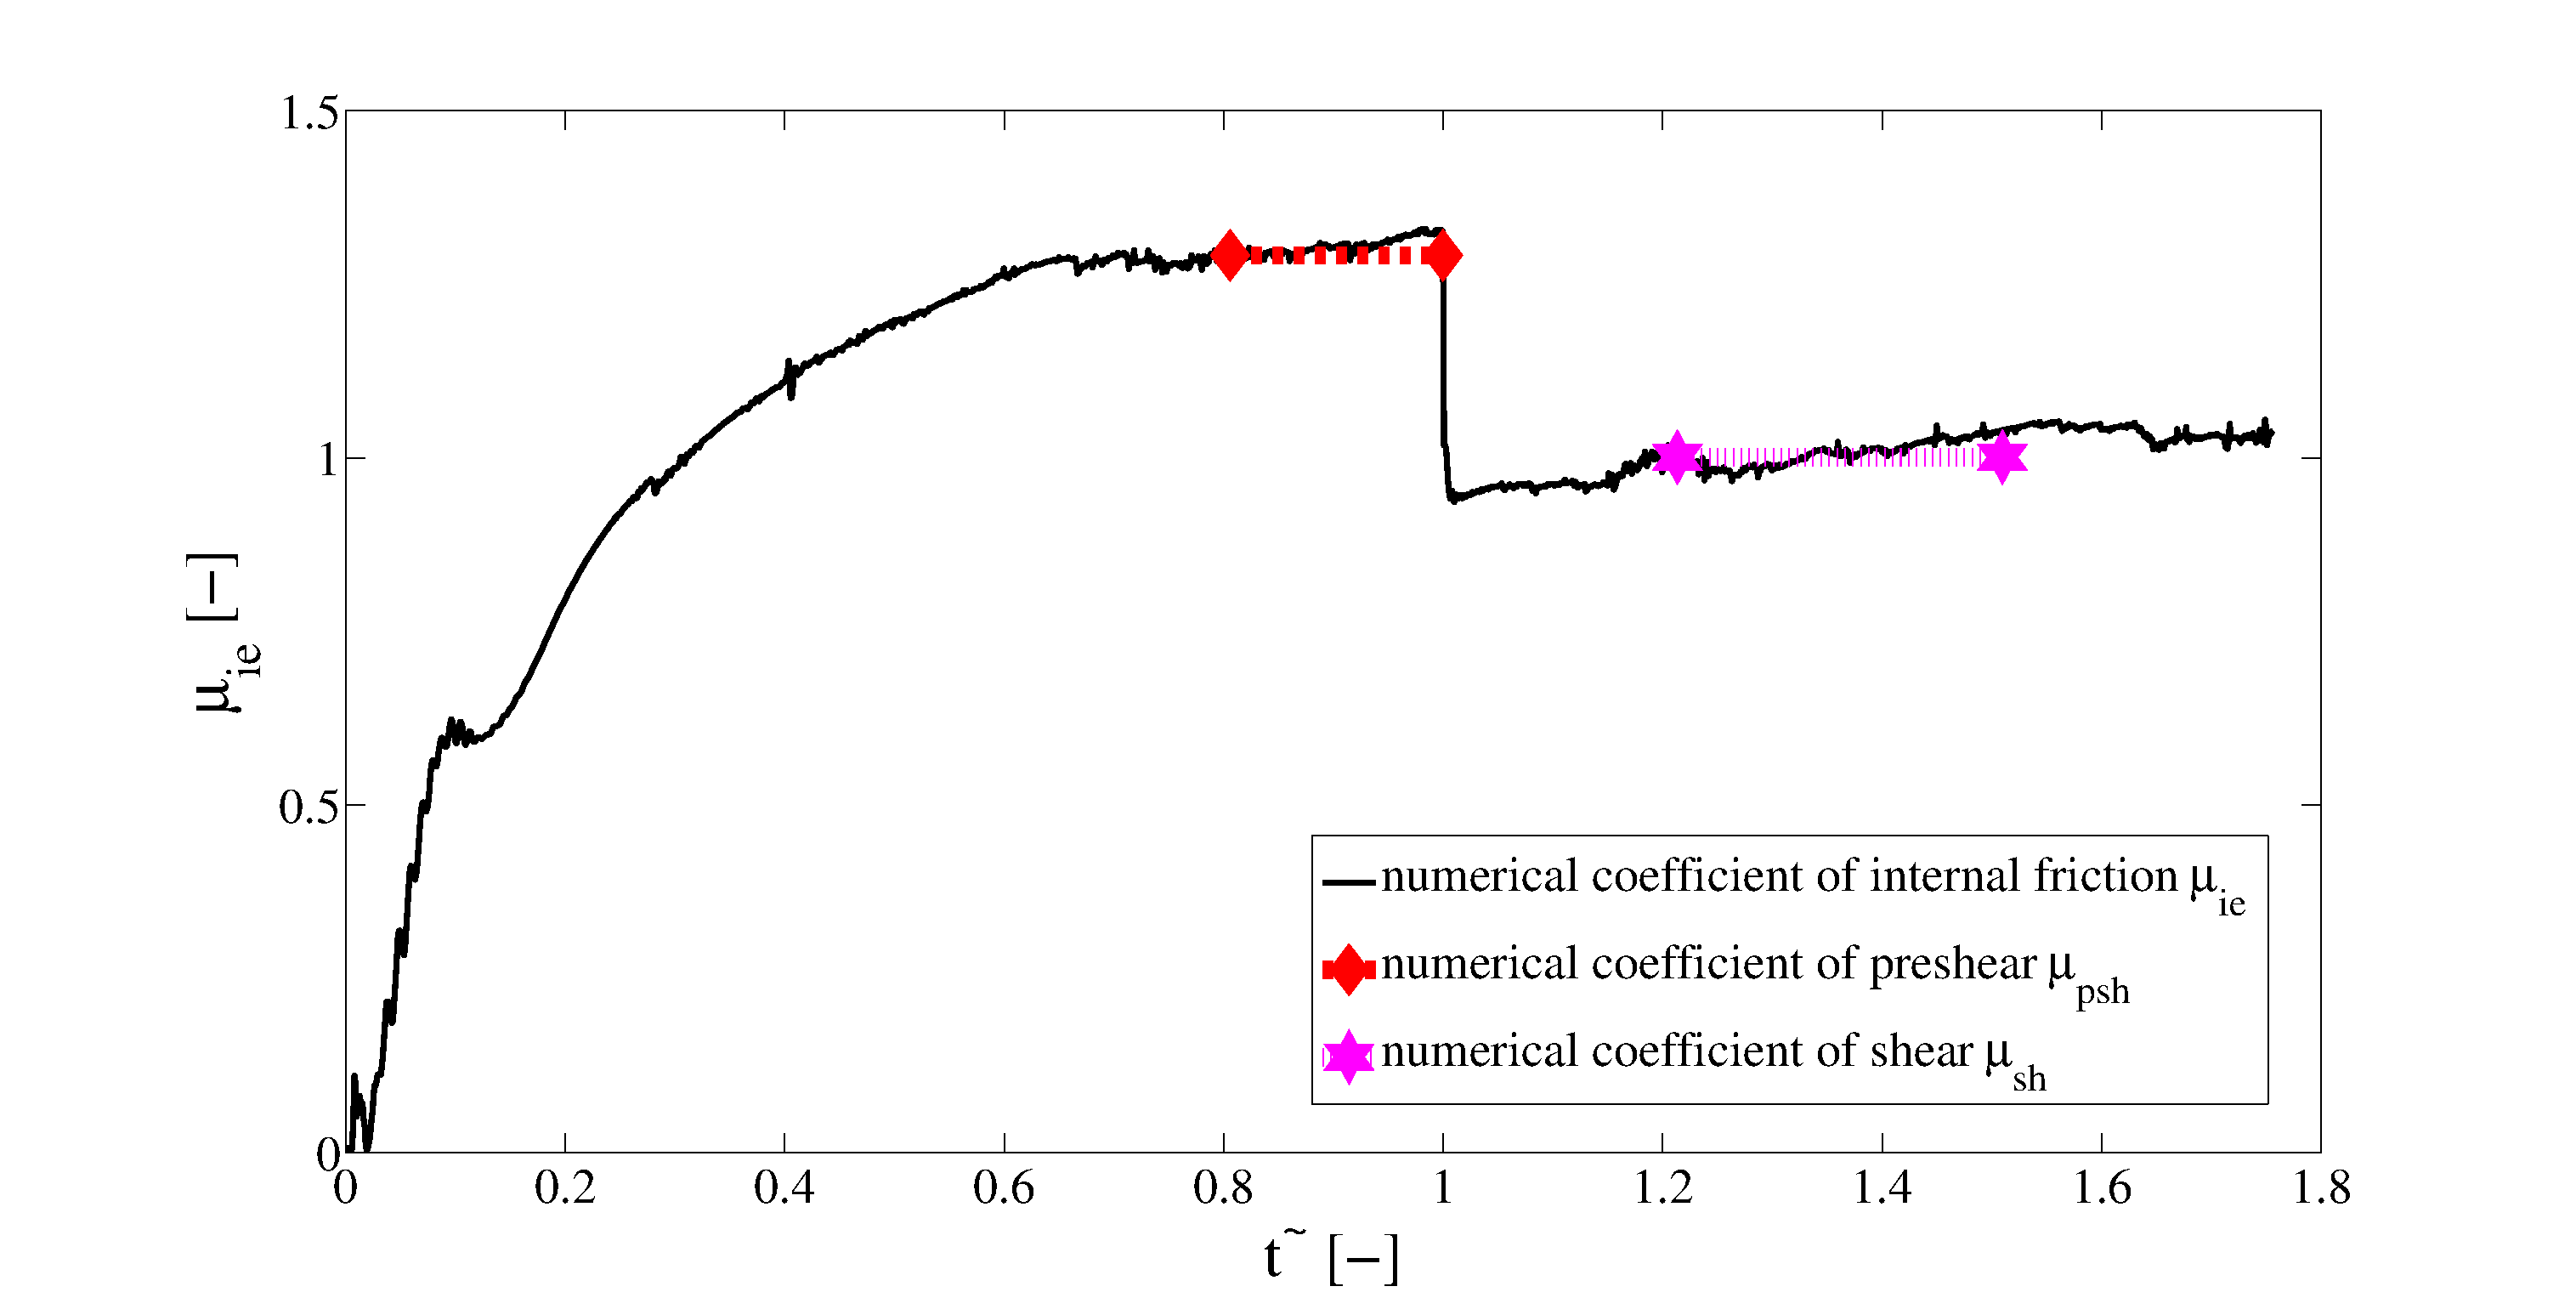
\includegraphics[width=\textwidth]{21simexample}
%         \caption{Numerical shear-cell tester stress path - $\sigma_n = 10000
%         ~Pa$}
%         \label{fig:21simexample} 
%     \end{subfigure}
%     \caption[Stress path]{Experimental and numerical samples of the stress path
%     for the Schulze ring shear cell tester.
% 	Time was normalized: $\tilde{t} = t/t_{change}$, where $t_{change}$ is the
% 	point in time at which the normal stress ($\sigma_n$) was modified during the
% 	tests.
% 	Until $\tilde{t}=1$, the $\sigma_n$ was kept constant at 10,000 Pa. 
% 	In Fig. \ref{fig:20experimental}, 
%  	a plateau was reached at $\tilde{t}~=0.91$.
% 	The coefficient of pre-shear (\ac{mupsh}) was calculated as the average of the
% 	coefficient of internal friction ($\mu_{ie}$) in this first plateau.
% 	At $\tilde{t}=1$, the $\sigma_n$ was reduced to $80 \%$ of its initial
% 	value, and soon after
% 	a second plateau developed.
% 	We obtained the coefficient of
% 	shear ($ \mu_{sh}$) as the average of $\mu_{ie}$ in this second plateau.
% 	The stress paths agree well, especially the plateaux.
% 	They were clearly relevant because
% 	the values representative of the bulk behaviours 
% 	were collected there.}
%     \label{fig:40experimentalsimulation}
% \end{figure}
Each \acs{SCT} simulation gave three of the \texit{bulk values} indicated in
Table \ref{tab:14bulkvalues}.
The first bulk value (\acs{rhob}) was provided directly. 
For correctly performed simulations, we
observed a stress path as the example in Fig. \ref{fig:021simexample}.
Time was normalized: $\tilde{t} = t/t_{change}$, where $t_{change}$ is the
point in time at which the normal stress (\acs{sigman}) was modified during the
tests.
Until $\tilde{t}=1$, the \acs{sigman} was kept constant at 10,000 Pa.
In Fig. \ref{fig:020experimental},
a plateau was reached at $\tilde{t}~=0.91$.
The coefficient of pre-shear (\acs{mupsh}) was calculated as the average of the
coefficient of internal friction (\acs{muie}) in this first plateau.
At $\tilde{t}=1$, the \acs{sigman} was reduced to $80 \%$ of its initial
value, and soon after
a second plateau developed.
We obtained the coefficient of
shear (\acs{mush}) as the average of \acs{muie} in this second plateau.
The stress paths between Fig. \ref{fig:007shearcellsim} and Fig.
\ref{fig:020experimental} agree well, especially the plateaux.
They were clearly relevant because
the values representative of the bulk behaviours were collected there.\\
Together with the value from the \acs{AoR} simulation, we were able to define
the numerical bulk behaviour.\\
All the results in this chapter are pure \acs{DEM}, so they shoould be
materials agnostic, given the same particle distribution, see
Section \ref{subsec:reliabilityconsiderations}.


%*-*-*-*-*-%*-*-*-*-*-%*-*-*-*-*-%*-*-*-*-*-%*-*-*-*-*-%*-*-*-*-*-%*-*-*-*-*-%*-*-*-*-*-%*-*-*-*-*-
%*-*-*-*-*-%*-*-*-*-*-%*-*-*-*-*-%*-*-*-*-*-%*-*-*-*-*-%*-*-*-*-*-%*-*-*-*-*-%*-*-*-*-*-%*-*-*-*-*-

\section{Influence of variations of input parameters}
\label{sec:influence}

In total, 2,400 shear cell and 400 static \acs{AoR} simulations 
were run with
the parameter combinations described in Table
\ref{tab:10DEMVariableinputvalues} with different particle size
distributions for the various materials analyzed.
The computational time amounted to 1 hour with 32 AMD cores for a benchmark
shear-cell simulation and to 9 hours for a benchmark \acs{AoR} simulation, both with
50,000 particles.
Simulations with larger \acs{dCylDp} required more time (e.g., about 12 hours for
the shear cell with 400,000 particles ). \\
To better understand the effect of the variation of the input parameters, nine
\acs{SCT} simulations have been selected, and their stress paths shown in Fig.
\ref{fig:136comparisonfrictioncoefficients}.

\begin{sidewaysfigure}[h]
\centering
\definecolor{mycolor1}{rgb}{0.00000,0.75000,0.75000}%
\definecolor{mycolor2}{rgb}{0.75000,0.00000,0.75000}%
\definecolor{mycolor3}{rgb}{0.75000,0.75000,0.00000}%
%
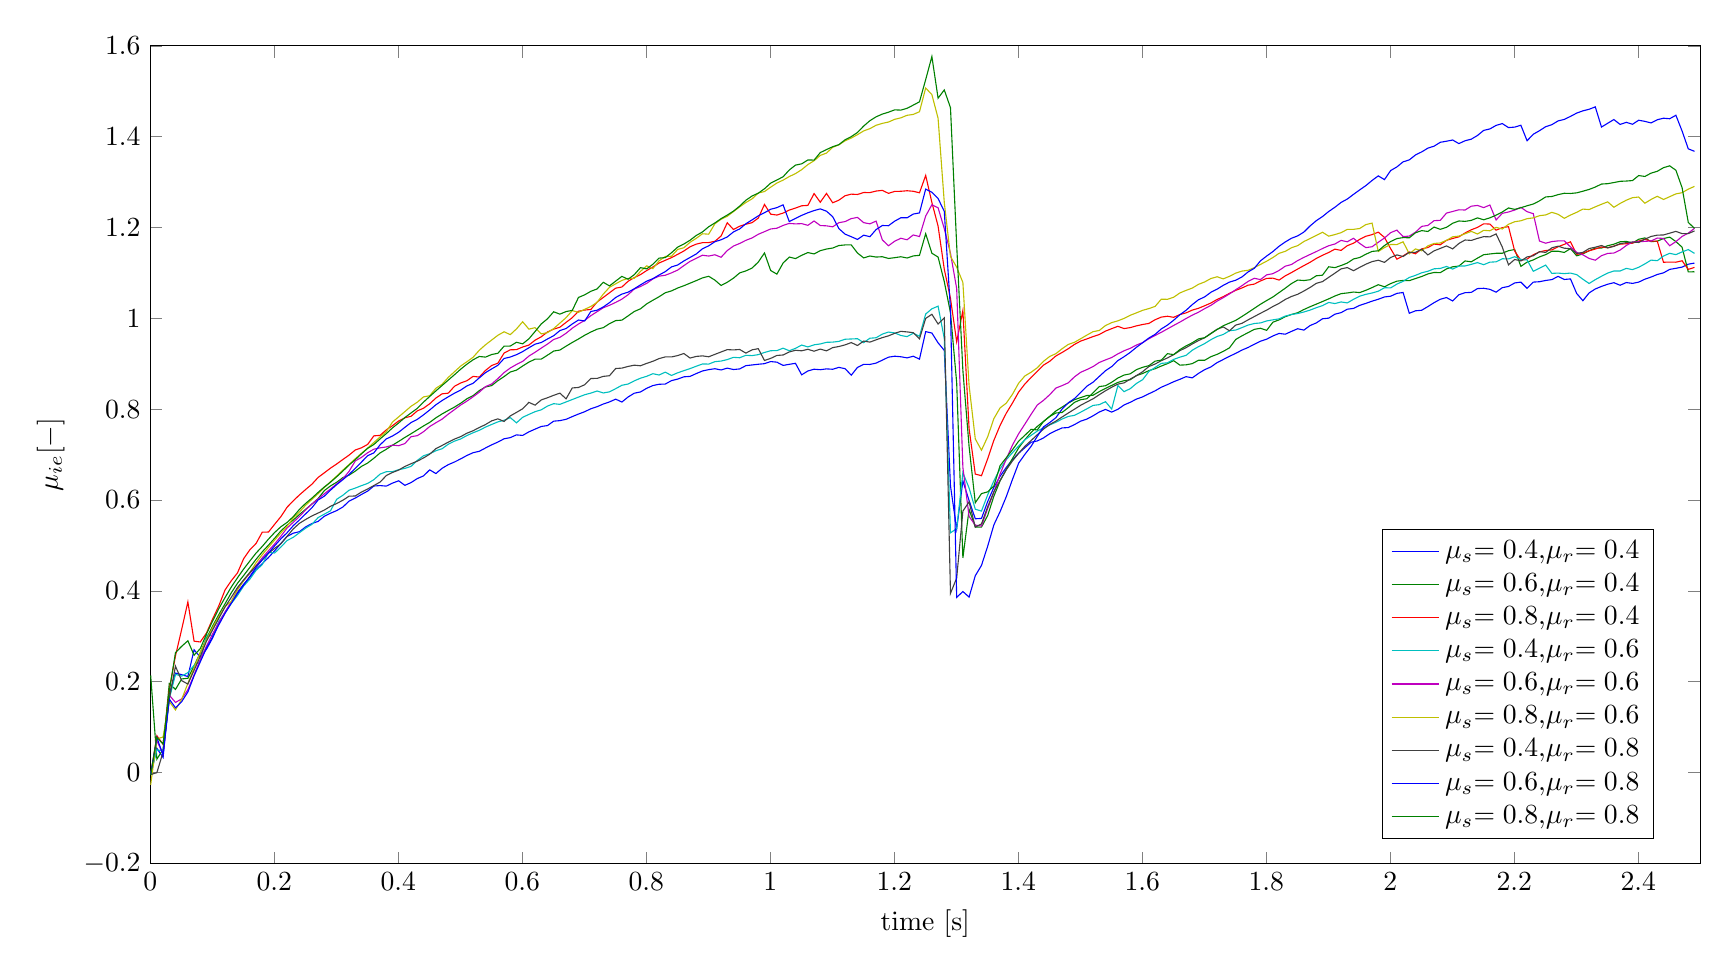
\begin{tikzpicture}

\begin{axis}[%
width=7.75in,
height=4.087734375in,
scale only axis,
xmin=0,
xmax=2.5,
xlabel={time [s]},
ymin=-0.2,
ymax=1.6,
ylabel={$\mu{}_{\text{ie}}\text{ [-]}$},
legend style={at={(0.97,0.03)},anchor=south east,draw=black,fill=white,legend cell align=left}
]
\addplot [color=blue,solid]
  table[row sep=crcr]{0.000714	-0.00509579883769\\
0.010714	0.0534680928292116\\
0.020714	0.0331095920407992\\
0.030714	0.17232132518135\\
0.040714	0.218901129096368\\
0.050714	0.215443198964465\\
0.060714	0.211303065989195\\
0.070714	0.270163982801088\\
0.080714	0.254119028162283\\
0.090714	0.271413411642901\\
0.100714	0.296517956036224\\
0.110714	0.329348063356903\\
0.120714	0.3531280148126\\
0.130714	0.373885977795794\\
0.140714	0.396568146590994\\
0.150714	0.414503178134599\\
0.160714	0.430230804569287\\
0.170714	0.446907091277694\\
0.180714	0.45998978127949\\
0.190714	0.473380863013444\\
0.200714	0.488256611290102\\
0.210714	0.504324944077742\\
0.220714	0.519627145671556\\
0.230714	0.526985537610999\\
0.240714	0.530284491378493\\
0.250714	0.540805431799351\\
0.260714	0.548127939079064\\
0.270714	0.552889754213776\\
0.280714	0.564076066912224\\
0.290714	0.570847422201881\\
0.300714	0.57670581211076\\
0.310714	0.584529218956066\\
0.320714	0.597580802590739\\
0.330714	0.604187706119813\\
0.340714	0.612270270304984\\
0.350714	0.619624285415107\\
0.360714	0.630813109882012\\
0.370714	0.631747257548671\\
0.380714	0.630609127401333\\
0.390714	0.637158227987776\\
0.400714	0.642305602434685\\
0.410714	0.632297013879975\\
0.420714	0.638383666118271\\
0.430714	0.647180604253621\\
0.440714	0.653004312523169\\
0.450714	0.666356803133989\\
0.460714	0.658243423578905\\
0.470714	0.669770448499043\\
0.480714	0.677816006532952\\
0.490714	0.68364776757073\\
0.500714	0.690500789460526\\
0.510714	0.698000685707458\\
0.520714	0.704113937277353\\
0.530714	0.707253206583718\\
0.540714	0.714518335196073\\
0.550714	0.721435834933235\\
0.560714	0.727573618575959\\
0.570714	0.734783024051892\\
0.580714	0.737335677976955\\
0.590714	0.743391426597188\\
0.600714	0.742168727400266\\
0.610714	0.749992509222831\\
0.620714	0.756072317548931\\
0.630714	0.761889794116546\\
0.640714	0.763855194844798\\
0.650714	0.773599350969769\\
0.660714	0.774766191629544\\
0.670714	0.777670296554887\\
0.680714	0.783632038407547\\
0.690714	0.789260497449855\\
0.700714	0.794369507974474\\
0.710714	0.800894365531896\\
0.720714	0.805443728671449\\
0.730714	0.811314624102451\\
0.740714	0.815947784944546\\
0.750714	0.822035465557335\\
0.760714	0.815671822027577\\
0.770714	0.826780488215157\\
0.780714	0.835120525604965\\
0.790714	0.837900757461473\\
0.800714	0.845961351625292\\
0.810714	0.851963521808982\\
0.820714	0.854832623158509\\
0.830714	0.855272655056821\\
0.840714	0.862829655225475\\
0.850714	0.866230024574124\\
0.860714	0.871220099931663\\
0.870714	0.872159804689208\\
0.880714	0.878403961425131\\
0.890714	0.884084869910048\\
0.900714	0.887011707711202\\
0.910714	0.889046200918384\\
0.920714	0.886335034466847\\
0.930714	0.890358275400011\\
0.940714	0.887250173465276\\
0.950714	0.888576435468835\\
0.960714	0.895805954986452\\
0.970714	0.897317958866629\\
0.980714	0.898878907398564\\
0.990714	0.900159250225404\\
1.000714	0.904801965968737\\
1.010714	0.903488008282866\\
1.020714	0.896316802048786\\
1.030714	0.898748612781487\\
1.040714	0.900916457862755\\
1.050714	0.875623509389394\\
1.060714	0.884055496287106\\
1.070714	0.887934911981697\\
1.080714	0.886882874325874\\
1.090714	0.888678887673099\\
1.100714	0.887859254522448\\
1.110714	0.892000974036151\\
1.120714	0.889128223211208\\
1.130714	0.874851717575083\\
1.140714	0.891952871609047\\
1.150714	0.898600208422586\\
1.160714	0.898443938721618\\
1.170714	0.901436624747713\\
1.180714	0.907847063631378\\
1.190714	0.914495879850376\\
1.200714	0.916587167879131\\
1.210714	0.915393610750444\\
1.220714	0.912920774623607\\
1.230714	0.916511287727268\\
1.240714	0.910140034766896\\
1.250714	0.970721483303378\\
1.260714	0.967609755688568\\
1.270714	0.946005030871829\\
1.280714	0.929446911910183\\
1.290714	0.630971388983964\\
1.300714	0.536199893385498\\
1.310714	0.642093479569319\\
1.320714	0.598838025672303\\
1.330714	0.558675776130121\\
1.340714	0.559453664988814\\
1.350714	0.59660028684968\\
1.360714	0.627770239265196\\
1.370714	0.652175957998672\\
1.380714	0.671840413802697\\
1.390714	0.688837085113224\\
1.400714	0.702970714016025\\
1.410714	0.715177529796251\\
1.420714	0.727139690232313\\
1.430714	0.73000430772133\\
1.440714	0.736667234674697\\
1.450714	0.745844337764252\\
1.460714	0.752689480141049\\
1.470714	0.758654354833069\\
1.480714	0.759573082771938\\
1.490714	0.766021691517448\\
1.500714	0.773646722792608\\
1.510714	0.7781972222756\\
1.520714	0.785393141326219\\
1.530714	0.793734658971056\\
1.540714	0.79939482134002\\
1.550714	0.793535784130619\\
1.560714	0.79977430762828\\
1.570714	0.809238586659696\\
1.580714	0.81518794661213\\
1.590714	0.822173830676136\\
1.600714	0.827070574278688\\
1.610714	0.833885548298572\\
1.620714	0.840337293164947\\
1.630714	0.848286902889703\\
1.640714	0.854132020920344\\
1.650714	0.860383338946045\\
1.660714	0.865732852794938\\
1.670714	0.871600212554195\\
1.680714	0.868944687537408\\
1.690714	0.878713838515599\\
1.700714	0.886969659694277\\
1.710714	0.892956145500708\\
1.720714	0.902486304677254\\
1.730714	0.909374395646162\\
1.740714	0.916362630380352\\
1.750714	0.922819914207574\\
1.760714	0.929993108988723\\
1.770714	0.935825864119734\\
1.780714	0.942811703609011\\
1.790714	0.949584735064027\\
1.800714	0.954099055253109\\
1.810714	0.961213635372177\\
1.820714	0.966710682435955\\
1.830714	0.965059899305057\\
1.840714	0.971250088837408\\
1.850714	0.977098942163975\\
1.860714	0.974071901950919\\
1.870714	0.984090652407739\\
1.880714	0.989872472885078\\
1.890714	0.999022671521152\\
1.900714	1.00035963741201\\
1.910714	1.00910226443509\\
1.920714	1.01251550437621\\
1.930714	1.02006256985342\\
1.940714	1.02183331437496\\
1.950714	1.02848550293083\\
1.960714	1.03290612655398\\
1.970714	1.03780927734759\\
1.980714	1.04199375192816\\
1.990714	1.04704103551978\\
2.000714	1.04872618745521\\
2.010714	1.05492974121387\\
2.020714	1.05684458893813\\
2.030714	1.01110000057843\\
2.040714	1.01656271723243\\
2.050714	1.01775929446251\\
2.060714	1.02586867379108\\
2.070714	1.03450700847944\\
2.080714	1.0419214267457\\
2.090714	1.04575153861802\\
2.100714	1.03815747864415\\
2.110714	1.05185038533059\\
2.120714	1.05644793626896\\
2.130714	1.0571164529606\\
2.140714	1.06548625156804\\
2.150714	1.06616680520678\\
2.160714	1.06381676185824\\
2.170714	1.05757989757961\\
2.180714	1.06749154228156\\
2.190714	1.07015309825761\\
2.200714	1.07789441134089\\
2.210714	1.07974048204779\\
2.220714	1.06601087988902\\
2.230714	1.07972594427685\\
2.240714	1.08061069133358\\
2.250714	1.08333528859251\\
2.260714	1.08526374828382\\
2.270714	1.09231338075482\\
2.280714	1.08551782593483\\
2.290714	1.08680408607424\\
2.300714	1.05471266775981\\
2.310714	1.03878159293376\\
2.320714	1.05585512792985\\
2.330714	1.06462422108682\\
2.340714	1.07025381488061\\
2.350714	1.07506067298082\\
2.360714	1.07844057360687\\
2.370714	1.07283433281405\\
2.380714	1.07878818014558\\
2.390714	1.07690917086936\\
2.400714	1.07970351025739\\
2.410714	1.08614331477725\\
2.420714	1.09090419824393\\
2.430714	1.09646668380713\\
2.440714	1.10010318872083\\
2.450714	1.10775290319132\\
2.460714	1.11009501464969\\
2.470714	1.11281078026261\\
2.480714	1.11916916259807\\
2.490714	1.12168161874395\\
};
\addlegendentry{$\mu{}_{\text{s}}\text{ = 0.4, }\mu{}_{\text{r}}\text{ = 0.4}$};

\addplot [color=black!50!green,solid]
  table[row sep=crcr]{0.000714	0.213560655526166\\
0.010714	0.0293429501025455\\
0.020714	0.0512119473555436\\
0.030714	0.196060184707133\\
0.040714	0.182932154101924\\
0.050714	0.20603572270319\\
0.060714	0.207449130848211\\
0.070714	0.23487831447985\\
0.080714	0.263838066926285\\
0.090714	0.29558956133881\\
0.100714	0.322711219850743\\
0.110714	0.347908284345503\\
0.120714	0.371688230882589\\
0.130714	0.395698030090412\\
0.140714	0.416651932789184\\
0.150714	0.433928985505918\\
0.160714	0.451711206428602\\
0.170714	0.469441832649821\\
0.180714	0.485949978771121\\
0.190714	0.500533046611371\\
0.200714	0.515903974107036\\
0.210714	0.531875923748354\\
0.220714	0.544539160808956\\
0.230714	0.555788458314853\\
0.240714	0.568220513739984\\
0.250714	0.579593501961628\\
0.260714	0.59100813115091\\
0.270714	0.603094419516489\\
0.280714	0.620562463383241\\
0.290714	0.630979208328822\\
0.300714	0.639076509591338\\
0.310714	0.64934596605447\\
0.320714	0.654774193590083\\
0.330714	0.663597289642089\\
0.340714	0.673981379958936\\
0.350714	0.681439590100422\\
0.360714	0.692024878936752\\
0.370714	0.703635178392642\\
0.380714	0.711631742697095\\
0.390714	0.7206964473525\\
0.400714	0.728979494989245\\
0.410714	0.737768181383373\\
0.420714	0.745964586778891\\
0.430714	0.754392747610772\\
0.440714	0.762979825206864\\
0.450714	0.770850004049894\\
0.460714	0.780875882172893\\
0.470714	0.789473235366767\\
0.480714	0.797147128857903\\
0.490714	0.804583604599601\\
0.500714	0.813048768084088\\
0.510714	0.822826047924798\\
0.520714	0.829742311989724\\
0.530714	0.840886946122784\\
0.540714	0.848866598653677\\
0.550714	0.851901590205576\\
0.560714	0.862703587011082\\
0.570714	0.871790942495533\\
0.580714	0.88181831148187\\
0.590714	0.885925100543936\\
0.600714	0.895033010529364\\
0.610714	0.903594331590822\\
0.620714	0.910075277368412\\
0.630714	0.910189974508843\\
0.640714	0.918863152947194\\
0.650714	0.927930864555038\\
0.660714	0.930151480148441\\
0.670714	0.938704341821557\\
0.680714	0.946875612422142\\
0.690714	0.954483927747892\\
0.700714	0.962691198730688\\
0.710714	0.969856886164817\\
0.720714	0.976066596047645\\
0.730714	0.979436750843874\\
0.740714	0.988211545747416\\
0.750714	0.995048860062346\\
0.760714	0.995977380982617\\
0.770714	1.00537318678673\\
0.780714	1.01504045876563\\
0.790714	1.02094037300079\\
0.800714	1.03181617725852\\
0.810714	1.03982283981893\\
0.820714	1.04752242685297\\
0.830714	1.05628980806893\\
0.840714	1.06036368916556\\
0.850714	1.06674901576418\\
0.860714	1.07175006086857\\
0.870714	1.07741434294259\\
0.880714	1.08304276997723\\
0.890714	1.08901164503882\\
0.900714	1.09257248270535\\
0.910714	1.08414700852667\\
0.920714	1.07229869441107\\
0.930714	1.07947657027964\\
0.940714	1.08839334538035\\
0.950714	1.09999633656638\\
0.960714	1.10441129959343\\
0.970714	1.11065221629304\\
0.980714	1.12389290475987\\
0.990714	1.1438634939387\\
1.000714	1.10526735006342\\
1.010714	1.09732656098848\\
1.020714	1.12162392783813\\
1.030714	1.13490240809247\\
1.040714	1.13151503218799\\
1.050714	1.13870771828232\\
1.060714	1.14477474172096\\
1.070714	1.14174141004381\\
1.080714	1.14897453258725\\
1.090714	1.15252679143259\\
1.100714	1.15475518252618\\
1.110714	1.160267129737\\
1.120714	1.16159741312801\\
1.130714	1.16160454999045\\
1.140714	1.14379079825651\\
1.150714	1.13300373261847\\
1.160714	1.13719096631706\\
1.170714	1.13485892846022\\
1.180714	1.13566522883251\\
1.190714	1.13182370638024\\
1.200714	1.13351957201777\\
1.210714	1.13556636443528\\
1.220714	1.13285780376567\\
1.230714	1.13742618872529\\
1.240714	1.13863431202093\\
1.250714	1.18634497850309\\
1.260714	1.14333706243455\\
1.270714	1.13486010313866\\
1.280714	1.08085592364244\\
1.290714	1.01221671684425\\
1.300714	0.858100340077299\\
1.310714	0.472425905761874\\
1.320714	0.579192838263399\\
1.330714	0.540668858797082\\
1.340714	0.540209630467532\\
1.350714	0.565911883364001\\
1.360714	0.608325010941382\\
1.370714	0.641984603854944\\
1.380714	0.66734661887118\\
1.390714	0.691285456110209\\
1.400714	0.71480199686042\\
1.410714	0.732795919328275\\
1.420714	0.748543134785227\\
1.430714	0.761931396554675\\
1.440714	0.772861594797774\\
1.450714	0.784135365283967\\
1.460714	0.796076465424832\\
1.470714	0.804489757759484\\
1.480714	0.813369832596451\\
1.490714	0.820851004359915\\
1.500714	0.825537009061934\\
1.510714	0.830017108623587\\
1.520714	0.830694938156785\\
1.530714	0.838650078522053\\
1.540714	0.845726490041342\\
1.550714	0.852294554174921\\
1.560714	0.85897386095789\\
1.570714	0.862678582024091\\
1.580714	0.864894866424798\\
1.590714	0.874077582255426\\
1.600714	0.878583393251238\\
1.610714	0.88487745572075\\
1.620714	0.889028237838307\\
1.630714	0.894929346313285\\
1.640714	0.900277898751135\\
1.650714	0.906776548590127\\
1.660714	0.896955408693159\\
1.670714	0.897619021033981\\
1.680714	0.900263763605151\\
1.690714	0.907601222396063\\
1.700714	0.907653188606608\\
1.710714	0.915531974421158\\
1.720714	0.92070265939976\\
1.730714	0.927273114169158\\
1.740714	0.935004244608058\\
1.750714	0.953331944154035\\
1.760714	0.961461012751312\\
1.770714	0.968405571735149\\
1.780714	0.975708832791969\\
1.790714	0.978109202064186\\
1.800714	0.973593190662096\\
1.810714	0.991439182749909\\
1.820714	0.996641330795992\\
1.830714	1.00351835479985\\
1.840714	1.00847486497973\\
1.850714	1.01235470090535\\
1.860714	1.01936724596622\\
1.870714	1.02555058504905\\
1.880714	1.03120984358631\\
1.890714	1.0369894226191\\
1.900714	1.04279498563779\\
1.910714	1.04911727836757\\
1.920714	1.05432233951618\\
1.930714	1.05583091357215\\
1.940714	1.05788161946537\\
1.950714	1.05666959968022\\
1.960714	1.06172531828565\\
1.970714	1.06767640391207\\
1.980714	1.07400087266035\\
1.990714	1.06941310551803\\
2.000714	1.07650557521168\\
2.010714	1.08180586147957\\
2.020714	1.08347974044797\\
2.030714	1.08289759745893\\
2.040714	1.08758269357378\\
2.050714	1.09206558714222\\
2.060714	1.09774821320679\\
2.070714	1.10102277490815\\
2.080714	1.10051940234327\\
2.090714	1.10876480578012\\
2.100714	1.1134213764009\\
2.110714	1.11510320403855\\
2.120714	1.1263294695223\\
2.130714	1.12443433741964\\
2.140714	1.13256225455555\\
2.150714	1.14003187695375\\
2.160714	1.14169293994873\\
2.170714	1.14320451973778\\
2.180714	1.14326888561591\\
2.190714	1.14884652601979\\
2.200714	1.1515472911448\\
2.210714	1.11440576057613\\
2.220714	1.12372764524141\\
2.230714	1.12855928874812\\
2.240714	1.13525058411757\\
2.250714	1.1402872683548\\
2.260714	1.14769556030967\\
2.270714	1.14774770207867\\
2.280714	1.14504394588199\\
2.290714	1.15355291244276\\
2.300714	1.1376194066344\\
2.310714	1.14174259259056\\
2.320714	1.14880635160394\\
2.330714	1.15456218702338\\
2.340714	1.15463978299508\\
2.350714	1.15984727707416\\
2.360714	1.16322832745323\\
2.370714	1.16851298723757\\
2.380714	1.16932364210806\\
2.390714	1.16574134842947\\
2.400714	1.17398964466936\\
2.410714	1.1770627488001\\
2.420714	1.16870033014965\\
2.430714	1.1698772853345\\
2.440714	1.1756572528262\\
2.450714	1.17880372710991\\
2.460714	1.16903489974456\\
2.470714	1.15665448174963\\
2.480714	1.10219323600458\\
2.490714	1.10251863265591\\
};
\addlegendentry{$\mu{}_{\text{s}}\text{ = 0.6, }\mu{}_{\text{r}}\text{ = 0.4}$};

\addplot [color=red,solid]
  table[row sep=crcr]{0.000714	-0.0049748921556281\\
0.010714	0.0810143936406392\\
0.020714	0.0621832726433686\\
0.030714	0.182712209072158\\
0.040714	0.256799207245693\\
0.050714	0.315196712113169\\
0.060714	0.375621673567208\\
0.070714	0.289213441595434\\
0.080714	0.287417541008914\\
0.090714	0.307099516665669\\
0.100714	0.338386100753474\\
0.110714	0.367392673514897\\
0.120714	0.402097093722472\\
0.130714	0.422195570253383\\
0.140714	0.439489522273633\\
0.150714	0.47089036109967\\
0.160714	0.490431097155672\\
0.170714	0.504377416503283\\
0.180714	0.529178564694041\\
0.190714	0.529494984702742\\
0.200714	0.546690489709869\\
0.210714	0.563352267964758\\
0.220714	0.584094710310725\\
0.230714	0.598350325311065\\
0.240714	0.611264583285339\\
0.250714	0.623206805328459\\
0.260714	0.634695656143741\\
0.270714	0.649563822238655\\
0.280714	0.65977438194985\\
0.290714	0.670088037285383\\
0.300714	0.67930274507127\\
0.310714	0.689202611635331\\
0.320714	0.698848203842125\\
0.330714	0.710098888216284\\
0.340714	0.714933040791589\\
0.350714	0.722476283611312\\
0.360714	0.741248722532235\\
0.370714	0.742290817684709\\
0.380714	0.754350229610683\\
0.390714	0.763597200992065\\
0.400714	0.774052056923035\\
0.410714	0.780940688323279\\
0.420714	0.784348759623364\\
0.430714	0.796214450021598\\
0.440714	0.802054392522988\\
0.450714	0.81182750630181\\
0.460714	0.824455799240043\\
0.470714	0.83372878876932\\
0.480714	0.835279492596548\\
0.490714	0.850379706595289\\
0.500714	0.857646231950533\\
0.510714	0.862546596262749\\
0.520714	0.872189019771901\\
0.530714	0.870673838370126\\
0.540714	0.885265415362942\\
0.550714	0.896141743369376\\
0.560714	0.90127625471667\\
0.570714	0.923460343229577\\
0.580714	0.930667344680557\\
0.590714	0.931058149993747\\
0.600714	0.936860728318168\\
0.610714	0.941113211467072\\
0.620714	0.951877256435512\\
0.630714	0.959445710727869\\
0.640714	0.969945940251683\\
0.650714	0.976203790000672\\
0.660714	0.980397971453808\\
0.670714	0.991128006896675\\
0.680714	1.00145964295198\\
0.690714	1.01563749711388\\
0.700714	1.01819057414511\\
0.710714	1.01951230196694\\
0.720714	1.03595088714855\\
0.730714	1.04593760414774\\
0.740714	1.05616645698553\\
0.750714	1.0664356325499\\
0.760714	1.06893089043315\\
0.770714	1.08157517147502\\
0.780714	1.08966350271972\\
0.790714	1.09625375238311\\
0.800714	1.10517042066622\\
0.810714	1.11298797099097\\
0.820714	1.12175156088793\\
0.830714	1.12774412499313\\
0.840714	1.13363443240834\\
0.850714	1.14082292209545\\
0.860714	1.14824833841633\\
0.870714	1.15753040378037\\
0.880714	1.16335297134641\\
0.890714	1.16659565162319\\
0.900714	1.16680778293176\\
0.910714	1.16956267633882\\
0.920714	1.1812424050896\\
0.930714	1.21037840287037\\
0.940714	1.19555026779431\\
0.950714	1.20281060651787\\
0.960714	1.20718904778253\\
0.970714	1.21063069662486\\
0.980714	1.22070488490393\\
0.990714	1.25071766008702\\
1.000714	1.22935353947724\\
1.010714	1.22736289216341\\
1.020714	1.2317035860473\\
1.030714	1.23835116744311\\
1.040714	1.24270678583776\\
1.050714	1.24777882532273\\
1.060714	1.24861983089162\\
1.070714	1.27469445491564\\
1.080714	1.2556528461714\\
1.090714	1.27491394408529\\
1.100714	1.25440326127845\\
1.110714	1.26009919278599\\
1.120714	1.26988177587924\\
1.130714	1.27338792408613\\
1.140714	1.27267475490079\\
1.150714	1.27695228707106\\
1.160714	1.27684091432747\\
1.170714	1.28016719397707\\
1.180714	1.28174842980434\\
1.190714	1.2751824754637\\
1.200714	1.27941326170244\\
1.210714	1.27970461078116\\
1.220714	1.28088237073327\\
1.230714	1.27973181024039\\
1.240714	1.27638477466022\\
1.250714	1.31453488375372\\
1.260714	1.25505918306525\\
1.270714	1.20316612234041\\
1.280714	1.10814942584664\\
1.290714	1.04407077515007\\
1.300714	0.948174115354437\\
1.310714	1.01699838264457\\
1.320714	0.757197920617424\\
1.330714	0.657066687307026\\
1.340714	0.653491738335835\\
1.350714	0.690733109391598\\
1.360714	0.731400612496569\\
1.370714	0.764123509042254\\
1.380714	0.791147352749028\\
1.390714	0.813603478238848\\
1.400714	0.83777128848385\\
1.410714	0.855386005518749\\
1.420714	0.869838529443791\\
1.430714	0.883359699391539\\
1.440714	0.896925669111555\\
1.450714	0.905375120623399\\
1.460714	0.917134294158475\\
1.470714	0.924815537828917\\
1.480714	0.933163401689213\\
1.490714	0.942555311823607\\
1.500714	0.949845197265823\\
1.510714	0.954699221366321\\
1.520714	0.959796782346589\\
1.530714	0.964371162430052\\
1.540714	0.971882915807888\\
1.550714	0.977266027147092\\
1.560714	0.982412476205198\\
1.570714	0.977417184087797\\
1.580714	0.979576832723201\\
1.590714	0.983416632531283\\
1.600714	0.986448856171474\\
1.610714	0.988772069048634\\
1.620714	0.996874993178208\\
1.630714	1.00267465962522\\
1.640714	1.00457641842375\\
1.650714	1.00219408982015\\
1.660714	1.00830669918076\\
1.670714	1.01198011364065\\
1.680714	1.01810904064947\\
1.690714	1.02204786994675\\
1.700714	1.02773327369758\\
1.710714	1.03368306910066\\
1.720714	1.04151494000812\\
1.730714	1.04776824747072\\
1.740714	1.05501078626715\\
1.750714	1.06154612572561\\
1.760714	1.06676393582339\\
1.770714	1.07294226567615\\
1.780714	1.07532199357795\\
1.790714	1.08225276672176\\
1.800714	1.08797020114324\\
1.810714	1.08842981438115\\
1.820714	1.08423761859266\\
1.830714	1.09350727573464\\
1.840714	1.10078184222269\\
1.850714	1.10852217006442\\
1.860714	1.11607494230033\\
1.870714	1.12339187334805\\
1.880714	1.13185128719838\\
1.890714	1.13883804460066\\
1.900714	1.14494640549375\\
1.910714	1.15227000738465\\
1.920714	1.14960357738717\\
1.930714	1.15990847748583\\
1.940714	1.16540351819037\\
1.950714	1.17382902740079\\
1.960714	1.18066723590754\\
1.970714	1.18433577135032\\
1.980714	1.18972378640844\\
1.990714	1.17811181499004\\
2.000714	1.15310527976178\\
2.010714	1.13020483419505\\
2.020714	1.13730791448496\\
2.030714	1.14600962702097\\
2.040714	1.14214446739987\\
2.050714	1.15283731343003\\
2.060714	1.1558636212575\\
2.070714	1.16344618989835\\
2.080714	1.16191465010451\\
2.090714	1.17168907748104\\
2.100714	1.1758321247307\\
2.110714	1.17939093295384\\
2.120714	1.1879538413829\\
2.130714	1.194931561704\\
2.140714	1.2002206688105\\
2.150714	1.20808282525452\\
2.160714	1.20749945603472\\
2.170714	1.19411955224042\\
2.180714	1.19962047323171\\
2.190714	1.20182410765893\\
2.200714	1.14816227887193\\
2.210714	1.12753055647767\\
2.220714	1.13044512374012\\
2.230714	1.13993576411545\\
2.240714	1.14633331116224\\
2.250714	1.14922992757222\\
2.260714	1.15075345959006\\
2.270714	1.15757336496944\\
2.280714	1.16289307816236\\
2.290714	1.16844147178719\\
2.300714	1.14079634149577\\
2.310714	1.14350894253178\\
2.320714	1.14869065217938\\
2.330714	1.15250922884396\\
2.340714	1.15709808451894\\
2.350714	1.15538866914809\\
2.360714	1.15911479883821\\
2.370714	1.16324707721118\\
2.380714	1.16420329659161\\
2.390714	1.16554605409792\\
2.400714	1.17014559853778\\
2.410714	1.17381538960743\\
2.420714	1.16990550435958\\
2.430714	1.17003325997865\\
2.440714	1.12348323907456\\
2.450714	1.12380456109141\\
2.460714	1.12356466550762\\
2.470714	1.12672177146689\\
2.480714	1.10777181999716\\
2.490714	1.11207012311904\\
};
\addlegendentry{$\mu{}_{\text{s}}\text{ = 0.8, }\mu{}_{\text{r}}\text{ = 0.4}$};

\addplot [color=mycolor1,solid]
  table[row sep=crcr]{0.000714	-0.00385229410814533\\
0.010714	0.0499785115496594\\
0.020714	0.047647643180244\\
0.030714	0.161988344430737\\
0.040714	0.216191030440153\\
0.050714	0.21220258557494\\
0.060714	0.219893178812936\\
0.070714	0.236011107829677\\
0.080714	0.245248601467972\\
0.090714	0.303349148007582\\
0.100714	0.301155607974163\\
0.110714	0.332917928498197\\
0.120714	0.35210435022597\\
0.130714	0.372022653028185\\
0.140714	0.389839246400756\\
0.150714	0.410708642706663\\
0.160714	0.425876978527758\\
0.170714	0.44510044677169\\
0.180714	0.457611242625664\\
0.190714	0.484506216912585\\
0.200714	0.483371176108634\\
0.210714	0.496322737235864\\
0.220714	0.510815156314658\\
0.230714	0.517860217614039\\
0.240714	0.528072687421084\\
0.250714	0.538061961558526\\
0.260714	0.546340685302515\\
0.270714	0.561207002656323\\
0.280714	0.568831009939838\\
0.290714	0.57625786893539\\
0.300714	0.60153811318418\\
0.310714	0.610430164563568\\
0.320714	0.621557122138091\\
0.330714	0.62624607159337\\
0.340714	0.631627623857826\\
0.350714	0.636523625595097\\
0.360714	0.644789332391093\\
0.370714	0.657062840924276\\
0.380714	0.662308988653426\\
0.390714	0.662415802725676\\
0.400714	0.666786271919637\\
0.410714	0.669592955807387\\
0.420714	0.674051402045459\\
0.430714	0.687130148255713\\
0.440714	0.697345935188599\\
0.450714	0.701790815871958\\
0.460714	0.708519876330817\\
0.470714	0.712860436624439\\
0.480714	0.722801406564737\\
0.490714	0.729601669817753\\
0.500714	0.734419032313144\\
0.510714	0.741897145156456\\
0.520714	0.748047846767626\\
0.530714	0.753390437343421\\
0.540714	0.760534487598292\\
0.550714	0.766336837075997\\
0.560714	0.77203631236503\\
0.570714	0.77556412362581\\
0.580714	0.781407230763829\\
0.590714	0.769860354019747\\
0.600714	0.782113123873429\\
0.610714	0.788449833754841\\
0.620714	0.794477823539332\\
0.630714	0.7986000377984\\
0.640714	0.806796577019118\\
0.650714	0.812106980908876\\
0.660714	0.810581914697409\\
0.670714	0.815883887475913\\
0.680714	0.821212876037651\\
0.690714	0.826542826212244\\
0.700714	0.831756909572844\\
0.710714	0.835392764378301\\
0.720714	0.840019380929323\\
0.730714	0.835692676686039\\
0.740714	0.838100520529519\\
0.750714	0.845143051069777\\
0.760714	0.852592029734329\\
0.770714	0.855328847428978\\
0.780714	0.86231258190079\\
0.790714	0.868137585806263\\
0.800714	0.872372605644109\\
0.810714	0.878101559995489\\
0.820714	0.875194638190052\\
0.830714	0.881479550823183\\
0.840714	0.874178117829269\\
0.850714	0.880100313499518\\
0.860714	0.884705174782365\\
0.870714	0.8893316321028\\
0.880714	0.894535048635616\\
0.890714	0.899465115785796\\
0.900714	0.899268362044407\\
0.910714	0.904582919369897\\
0.920714	0.90592894211875\\
0.930714	0.909161526994985\\
0.940714	0.914068265719804\\
0.950714	0.913219468793061\\
0.960714	0.918571454956759\\
0.970714	0.917902058957203\\
0.980714	0.920086355352491\\
0.990714	0.924807453535656\\
1.000714	0.928675957940117\\
1.010714	0.928894329488902\\
1.020714	0.934259429910664\\
1.030714	0.928621641446929\\
1.040714	0.93392365646779\\
1.050714	0.941155474481183\\
1.060714	0.937032490312642\\
1.070714	0.941698125871978\\
1.080714	0.94358305063115\\
1.090714	0.947171231951805\\
1.100714	0.947615263914008\\
1.110714	0.949236533564577\\
1.120714	0.953939653844684\\
1.130714	0.954541211321304\\
1.140714	0.955129291270126\\
1.150714	0.946428927270308\\
1.160714	0.956187030383001\\
1.170714	0.957233563519847\\
1.180714	0.965231874605589\\
1.190714	0.969764729843911\\
1.200714	0.967831703932399\\
1.210714	0.962237442082831\\
1.220714	0.959724642556846\\
1.230714	0.96717471033194\\
1.240714	0.960540695167412\\
1.250714	1.00946657967634\\
1.260714	1.02098695613441\\
1.270714	1.02681319296\\
1.280714	0.955637021045774\\
1.290714	0.527800306290507\\
1.300714	0.536900264849431\\
1.310714	0.660191067481282\\
1.320714	0.626425559756588\\
1.330714	0.579751241263025\\
1.340714	0.5756165557141\\
1.350714	0.611318390950185\\
1.360714	0.642352087272295\\
1.370714	0.668806172295475\\
1.380714	0.688696234264449\\
1.390714	0.704178235882265\\
1.400714	0.719037844966003\\
1.410714	0.732442096255493\\
1.420714	0.74227445070062\\
1.430714	0.75175563019929\\
1.440714	0.758510979232095\\
1.450714	0.765251934217018\\
1.460714	0.771063135660064\\
1.470714	0.778286909195578\\
1.480714	0.783975775852282\\
1.490714	0.786375263569139\\
1.500714	0.793377776932448\\
1.510714	0.800724665801271\\
1.520714	0.808267042211313\\
1.530714	0.809945159759215\\
1.540714	0.81651375827159\\
1.550714	0.800188129980059\\
1.560714	0.851954522182367\\
1.570714	0.838587081188684\\
1.580714	0.845163495723247\\
1.590714	0.856671375484207\\
1.600714	0.864985858513068\\
1.610714	0.883049721923985\\
1.620714	0.891687726985733\\
1.630714	0.900769284522802\\
1.640714	0.902103234785602\\
1.650714	0.909590786702668\\
1.660714	0.914521854963549\\
1.670714	0.91845862664792\\
1.680714	0.92976796803015\\
1.690714	0.93761823286752\\
1.700714	0.944477160904195\\
1.710714	0.952941231621469\\
1.720714	0.960055755826813\\
1.730714	0.964540613245873\\
1.740714	0.972697030977559\\
1.750714	0.974147217541521\\
1.760714	0.979495674548942\\
1.770714	0.985172795050744\\
1.780714	0.988579308066832\\
1.790714	0.989885182786915\\
1.800714	0.994239870255259\\
1.810714	0.996653732539677\\
1.820714	0.998766809172808\\
1.830714	1.00497470673375\\
1.840714	1.00828621333783\\
1.850714	1.01056458042837\\
1.860714	1.01397243855524\\
1.870714	1.01812857744169\\
1.880714	1.0233541744537\\
1.890714	1.02791970160949\\
1.900714	1.03495454575166\\
1.910714	1.03250439250688\\
1.920714	1.036033437118\\
1.930714	1.03397270680168\\
1.940714	1.04182903458063\\
1.950714	1.0487846326073\\
1.960714	1.05280966911929\\
1.970714	1.05577424211391\\
1.980714	1.05968172331938\\
1.990714	1.06730087329926\\
2.000714	1.06708324480884\\
2.010714	1.07531507475589\\
2.020714	1.08144574821993\\
2.030714	1.08999194533967\\
2.040714	1.09465358289845\\
2.050714	1.10019533784277\\
2.060714	1.1036374536774\\
2.070714	1.10900668317913\\
2.080714	1.1098616124559\\
2.090714	1.11420860263188\\
2.100714	1.10833645047435\\
2.110714	1.11498174877588\\
2.120714	1.11528112278973\\
2.130714	1.11884511463126\\
2.140714	1.12273737096366\\
2.150714	1.11810151136507\\
2.160714	1.12360259773274\\
2.170714	1.12440017277639\\
2.180714	1.13111043081712\\
2.190714	1.1308470235097\\
2.200714	1.13563602149218\\
2.210714	1.12955614246779\\
2.220714	1.12851302866137\\
2.230714	1.10366047426187\\
2.240714	1.11045348857953\\
2.250714	1.11715955064604\\
2.260714	1.09898667871779\\
2.270714	1.09958919611705\\
2.280714	1.09846148608078\\
2.290714	1.09962935150484\\
2.300714	1.09621864968102\\
2.310714	1.0860652795079\\
2.320714	1.07668638613575\\
2.330714	1.08514330045954\\
2.340714	1.09262175244995\\
2.350714	1.09969049114183\\
2.360714	1.10421309401922\\
2.370714	1.1041659087453\\
2.380714	1.1099873698643\\
2.390714	1.10721524229003\\
2.400714	1.11236110413052\\
2.410714	1.11985248486235\\
2.420714	1.12814120956207\\
2.430714	1.12693276399744\\
2.440714	1.13720100959945\\
2.450714	1.14311031872359\\
2.460714	1.14021644956218\\
2.470714	1.14621126379131\\
2.480714	1.15136335842795\\
2.490714	1.14302179855168\\
};
\addlegendentry{$\mu{}_{\text{s}}\text{ = 0.4, }\mu{}_{\text{r}}\text{ = 0.6}$};

\addplot [color=mycolor2,solid]
  table[row sep=crcr]{0.000714	-0.0040042400207269\\
0.010714	0.0698174689680346\\
0.020714	0.0405486252595229\\
0.030714	0.170350266325852\\
0.040714	0.154271435604026\\
0.050714	0.162117560654956\\
0.060714	0.182229044805257\\
0.070714	0.215038226904861\\
0.080714	0.248646034122246\\
0.090714	0.27837100868675\\
0.100714	0.305289584193405\\
0.110714	0.330157109564551\\
0.120714	0.353300581574703\\
0.130714	0.375785645208669\\
0.140714	0.404024538769416\\
0.150714	0.422472121153685\\
0.160714	0.438600984436424\\
0.170714	0.455652081499264\\
0.180714	0.472847499803011\\
0.190714	0.488283401346461\\
0.200714	0.503342950830179\\
0.210714	0.520184770522435\\
0.220714	0.538262440637771\\
0.230714	0.550834120538593\\
0.240714	0.56381563693553\\
0.250714	0.578180458798978\\
0.260714	0.591149474305815\\
0.270714	0.602303930776485\\
0.280714	0.613623147931561\\
0.290714	0.624157331493094\\
0.300714	0.635422110406276\\
0.310714	0.646807968825711\\
0.320714	0.663119038525003\\
0.330714	0.685968973647606\\
0.340714	0.693839754766021\\
0.350714	0.704090777209723\\
0.360714	0.711899850688154\\
0.370714	0.714815291642783\\
0.380714	0.716786885682982\\
0.390714	0.720808526276332\\
0.400714	0.719557845021286\\
0.410714	0.724261170143275\\
0.420714	0.739404215910937\\
0.430714	0.7416228800156\\
0.440714	0.750268264378826\\
0.450714	0.761719001041472\\
0.460714	0.770069076108444\\
0.470714	0.778047258963823\\
0.480714	0.788996123368181\\
0.490714	0.799003602750677\\
0.500714	0.809146960543608\\
0.510714	0.817614632584819\\
0.520714	0.82722317766244\\
0.530714	0.837389122521394\\
0.540714	0.849607805704476\\
0.550714	0.855432538611535\\
0.560714	0.867330894583086\\
0.570714	0.880527494547109\\
0.580714	0.890649218040393\\
0.590714	0.898434505847217\\
0.600714	0.905209202549803\\
0.610714	0.916840413361673\\
0.620714	0.925310497937856\\
0.630714	0.934483379798651\\
0.640714	0.943308333466055\\
0.650714	0.953441527322606\\
0.660714	0.958095447862452\\
0.670714	0.967132953620654\\
0.680714	0.978247114666761\\
0.690714	0.987480440497305\\
0.700714	0.995426627420197\\
0.710714	1.00589830315194\\
0.720714	1.01462312988454\\
0.730714	1.0232532971764\\
0.740714	1.02865265195911\\
0.750714	1.035035489389\\
0.760714	1.04220546361455\\
0.770714	1.05196548154445\\
0.780714	1.0645860694794\\
0.790714	1.07001706117265\\
0.800714	1.07697613246191\\
0.810714	1.08678638410601\\
0.820714	1.09283874118356\\
0.830714	1.09483823127364\\
0.840714	1.10007247739124\\
0.850714	1.10625838671871\\
0.860714	1.11604060034982\\
0.870714	1.12547275420024\\
0.880714	1.13208978710643\\
0.890714	1.13894275475273\\
0.900714	1.13709174396154\\
0.910714	1.13992667557546\\
0.920714	1.13447912532622\\
0.930714	1.14920170290356\\
0.940714	1.15913852499188\\
0.950714	1.16485652847699\\
0.960714	1.17178386631304\\
0.970714	1.1769879167765\\
0.980714	1.18501726943439\\
0.990714	1.19082216123607\\
1.000714	1.19674022981206\\
1.010714	1.19837062558856\\
1.020714	1.20451548946365\\
1.030714	1.20896885624447\\
1.040714	1.20793193679319\\
1.050714	1.20848589474097\\
1.060714	1.20474272863552\\
1.070714	1.21435855374586\\
1.080714	1.20427462519162\\
1.090714	1.20364600306422\\
1.100714	1.2015052482032\\
1.110714	1.21055957133419\\
1.120714	1.21300095106383\\
1.130714	1.21955024562283\\
1.140714	1.22222321818651\\
1.150714	1.2106458522134\\
1.160714	1.20802837652299\\
1.170714	1.21406191839877\\
1.180714	1.17279373795553\\
1.190714	1.15978018129945\\
1.200714	1.16979586414349\\
1.210714	1.1762340847464\\
1.220714	1.172978403854\\
1.230714	1.1835529899912\\
1.240714	1.1800966007111\\
1.250714	1.22524318780386\\
1.260714	1.25003032829831\\
1.270714	1.24339011966112\\
1.280714	1.19743680048194\\
1.290714	1.14309487021945\\
1.300714	1.0656322178666\\
1.310714	0.67153486359484\\
1.320714	0.563872563178524\\
1.330714	0.544660821733353\\
1.340714	0.542727586569013\\
1.350714	0.581310303115988\\
1.360714	0.616937041832773\\
1.370714	0.65701581346077\\
1.380714	0.690401691666785\\
1.390714	0.721060832534025\\
1.400714	0.746042266732997\\
1.410714	0.767122927796499\\
1.420714	0.78861329870895\\
1.430714	0.809156345374987\\
1.440714	0.819327371494994\\
1.450714	0.831841233712582\\
1.460714	0.846425740578009\\
1.470714	0.851846448512965\\
1.480714	0.858023995006099\\
1.490714	0.871146122469775\\
1.500714	0.881189702638041\\
1.510714	0.887177400676747\\
1.520714	0.893782308676128\\
1.530714	0.902815426322185\\
1.540714	0.908436403273788\\
1.550714	0.913690385435287\\
1.560714	0.921782926496893\\
1.570714	0.928602827699645\\
1.580714	0.933995955900858\\
1.590714	0.941233132962697\\
1.600714	0.9465973729236\\
1.610714	0.955052519362291\\
1.620714	0.962213245088421\\
1.630714	0.969221341669957\\
1.640714	0.976795202817558\\
1.650714	0.984362992298221\\
1.660714	0.991679281382819\\
1.670714	0.999596975875082\\
1.680714	1.00699271884345\\
1.690714	1.0135016582735\\
1.700714	1.0213097543458\\
1.710714	1.028511745848\\
1.720714	1.03779646322505\\
1.730714	1.04547148052678\\
1.740714	1.05384482619149\\
1.750714	1.06284830409738\\
1.760714	1.0718580208415\\
1.770714	1.08120620304358\\
1.780714	1.08808446316337\\
1.790714	1.08533341126491\\
1.800714	1.09572928380273\\
1.810714	1.09828251293221\\
1.820714	1.10540836139686\\
1.830714	1.11479312238659\\
1.840714	1.11849272808469\\
1.850714	1.12716738951612\\
1.860714	1.13414418041783\\
1.870714	1.14060355317239\\
1.880714	1.14690486425272\\
1.890714	1.15370099253584\\
1.900714	1.1598258916246\\
1.910714	1.16362557229658\\
1.920714	1.17154861144055\\
1.930714	1.16855196452508\\
1.940714	1.17622817527923\\
1.950714	1.16494312489948\\
1.960714	1.15560990722396\\
1.970714	1.15761392160543\\
1.980714	1.16749162196425\\
1.990714	1.17680373336707\\
2.000714	1.18867397629509\\
2.010714	1.19417784830211\\
2.020714	1.17994830501895\\
2.030714	1.18106401666436\\
2.040714	1.18959002260878\\
2.050714	1.20241598692813\\
2.060714	1.2045445833567\\
2.070714	1.21503592151456\\
2.080714	1.21572468869844\\
2.090714	1.231703016685\\
2.100714	1.23528543086182\\
2.110714	1.23894951830614\\
2.120714	1.23847394732371\\
2.130714	1.24687199087217\\
2.140714	1.24853257423775\\
2.150714	1.24375402637856\\
2.160714	1.24945582889221\\
2.170714	1.21659030190823\\
2.180714	1.23112101592517\\
2.190714	1.23409982678248\\
2.200714	1.2383540567921\\
2.210714	1.2442717132719\\
2.220714	1.23477178996425\\
2.230714	1.23042785684374\\
2.240714	1.17011342795373\\
2.250714	1.16536167115138\\
2.260714	1.16899706773228\\
2.270714	1.17045127728727\\
2.280714	1.17064878699033\\
2.290714	1.15714895897239\\
2.300714	1.14532955761865\\
2.310714	1.13974470995638\\
2.320714	1.13186157240356\\
2.330714	1.12793220508387\\
2.340714	1.13792669907728\\
2.350714	1.14290636114105\\
2.360714	1.1437252071169\\
2.370714	1.15021175155204\\
2.380714	1.16029803719143\\
2.390714	1.16817237131249\\
2.400714	1.16864634044916\\
2.410714	1.16942862561389\\
2.420714	1.17031782377224\\
2.430714	1.17672650593659\\
2.440714	1.1758971042201\\
2.450714	1.15982336967672\\
2.460714	1.16878172031127\\
2.470714	1.18031152543516\\
2.480714	1.18763075818391\\
2.490714	1.19814233995857\\
};
\addlegendentry{$\mu{}_{\text{s}}\text{ = 0.6, }\mu{}_{\text{r}}\text{ = 0.6}$};

\addplot [color=mycolor3,solid]
  table[row sep=crcr]{0.000714	-0.0269122570677535\\
0.010714	0.0741954684033824\\
0.020714	0.0780538759276238\\
0.030714	0.156327401815168\\
0.040714	0.137847787479753\\
0.050714	0.161109656158669\\
0.060714	0.196290108076076\\
0.070714	0.230695477245636\\
0.080714	0.26451338514003\\
0.090714	0.292343123722227\\
0.100714	0.319257172937811\\
0.110714	0.343662201586601\\
0.120714	0.365790407149931\\
0.130714	0.376533887606883\\
0.140714	0.4019389852213\\
0.150714	0.422672774979288\\
0.160714	0.440440425776527\\
0.170714	0.462135869117762\\
0.180714	0.479697717879268\\
0.190714	0.495871527037827\\
0.200714	0.511823180212966\\
0.210714	0.527516295619299\\
0.220714	0.542006778473931\\
0.230714	0.560718931813569\\
0.240714	0.573839474049407\\
0.250714	0.5885533140205\\
0.260714	0.601298900166299\\
0.270714	0.613922288028653\\
0.280714	0.627334014502557\\
0.290714	0.640176235509166\\
0.300714	0.652592627877673\\
0.310714	0.665798676533003\\
0.320714	0.678080793260609\\
0.330714	0.690844797762135\\
0.340714	0.702810992178628\\
0.350714	0.714405156452411\\
0.360714	0.726669024467368\\
0.370714	0.738839580941985\\
0.380714	0.750547749139035\\
0.390714	0.771623431915167\\
0.400714	0.783094235869346\\
0.410714	0.794578903676995\\
0.420714	0.806393235895016\\
0.430714	0.815287442799012\\
0.440714	0.826981997869835\\
0.450714	0.82954608635164\\
0.460714	0.846060606848029\\
0.470714	0.854778837303264\\
0.480714	0.869924629798118\\
0.490714	0.882448320116911\\
0.500714	0.894914938501807\\
0.510714	0.904410957133948\\
0.520714	0.914260836206857\\
0.530714	0.929615966059972\\
0.540714	0.941738809572287\\
0.550714	0.95217540421811\\
0.560714	0.962679230982425\\
0.570714	0.970330492550778\\
0.580714	0.964105276660931\\
0.590714	0.976747292311606\\
0.600714	0.992475371496447\\
0.610714	0.976186336083736\\
0.620714	0.979476336863364\\
0.630714	0.965688395248325\\
0.640714	0.96857338786672\\
0.650714	0.977409684310973\\
0.660714	0.989458401807057\\
0.670714	1.00155578502559\\
0.680714	1.0170348618045\\
0.690714	1.01310512998029\\
0.700714	1.01979705070827\\
0.710714	1.02618839212153\\
0.720714	1.03510070646249\\
0.730714	1.05335092740161\\
0.740714	1.06828268323116\\
0.750714	1.07595490289807\\
0.760714	1.08350454267162\\
0.770714	1.08784513219046\\
0.780714	1.08806347431669\\
0.790714	1.10334543575816\\
0.800714	1.11554403209139\\
0.810714	1.1094323926995\\
0.820714	1.1266177079629\\
0.830714	1.13612676298716\\
0.840714	1.13672355515168\\
0.850714	1.1517111005576\\
0.860714	1.15537509658878\\
0.870714	1.16746014296188\\
0.880714	1.17612232612407\\
0.890714	1.18616233153828\\
0.900714	1.18523272492837\\
0.910714	1.20815505890834\\
0.920714	1.21818299257215\\
0.930714	1.22470128715964\\
0.940714	1.23497320840412\\
0.950714	1.2453625073692\\
0.960714	1.2549804662633\\
0.970714	1.26302032123375\\
0.980714	1.27590667328884\\
0.990714	1.27912827894917\\
1.000714	1.28878762526463\\
1.010714	1.29783939521981\\
1.020714	1.30424872184245\\
1.030714	1.31216110614147\\
1.040714	1.31858354119957\\
1.050714	1.32731180222933\\
1.060714	1.33846638798456\\
1.070714	1.34700403280628\\
1.080714	1.3586888949453\\
1.090714	1.36377623283606\\
1.100714	1.37649788577876\\
1.110714	1.38198427875085\\
1.120714	1.39082946134986\\
1.130714	1.39684359913841\\
1.140714	1.40440383802446\\
1.150714	1.41266887450273\\
1.160714	1.4175979628031\\
1.170714	1.42503160120081\\
1.180714	1.42918685237534\\
1.190714	1.4321850624138\\
1.200714	1.43813404077429\\
1.210714	1.44146531011204\\
1.220714	1.44699691827788\\
1.230714	1.44893872348263\\
1.240714	1.45490370430847\\
1.250714	1.50706204091191\\
1.260714	1.4925501738567\\
1.270714	1.44045285216444\\
1.280714	1.25519144816343\\
1.290714	1.13627295575549\\
1.300714	1.11261138120129\\
1.310714	1.07900336817388\\
1.320714	0.852113207147153\\
1.330714	0.734495123641537\\
1.340714	0.709623640494404\\
1.350714	0.739172442108643\\
1.360714	0.779229346809492\\
1.370714	0.80281423834086\\
1.380714	0.813232611919852\\
1.390714	0.832876714916669\\
1.400714	0.857308274400218\\
1.410714	0.873183232130539\\
1.420714	0.881283814540948\\
1.430714	0.89114630349852\\
1.440714	0.905321596468519\\
1.450714	0.916006076284296\\
1.460714	0.922161261880969\\
1.470714	0.933034422020444\\
1.480714	0.942539713379253\\
1.490714	0.947258229226632\\
1.500714	0.955083703601005\\
1.510714	0.963087563075355\\
1.520714	0.970657385793719\\
1.530714	0.973283161080354\\
1.540714	0.984050718890142\\
1.550714	0.99054536260873\\
1.560714	0.994471463132736\\
1.570714	0.999868070760175\\
1.580714	1.00671684448895\\
1.590714	1.01208301406061\\
1.600714	1.01761698893294\\
1.610714	1.02147217939326\\
1.620714	1.02619086846569\\
1.630714	1.04207105231858\\
1.640714	1.04183547352773\\
1.650714	1.04648890543368\\
1.660714	1.05590051119252\\
1.670714	1.06155448453255\\
1.680714	1.06657263360091\\
1.690714	1.07480726639159\\
1.700714	1.08010420343102\\
1.710714	1.08761699896743\\
1.720714	1.0914862105673\\
1.730714	1.08687374872207\\
1.740714	1.09250302520138\\
1.750714	1.09947765746295\\
1.760714	1.10399067522653\\
1.770714	1.10576394837276\\
1.780714	1.111602991855\\
1.790714	1.1186844749133\\
1.800714	1.12580265428763\\
1.810714	1.13385526288855\\
1.820714	1.14309507945046\\
1.830714	1.14750388829998\\
1.840714	1.15537446330026\\
1.850714	1.15998670010067\\
1.860714	1.16909755804877\\
1.870714	1.17560288038812\\
1.880714	1.18245036311013\\
1.890714	1.18950839356638\\
1.900714	1.18090925296762\\
1.910714	1.18437693898545\\
1.920714	1.1885872986812\\
1.930714	1.19575474103462\\
1.940714	1.19589714684543\\
1.950714	1.19775887913891\\
1.960714	1.20639367734263\\
1.970714	1.20957394384727\\
1.980714	1.14720171282137\\
1.990714	1.15579536185581\\
2.000714	1.16257565692764\\
2.010714	1.16232642122258\\
2.020714	1.16850230205379\\
2.030714	1.14209205534178\\
2.040714	1.15280854127555\\
2.050714	1.14853218116403\\
2.060714	1.15962515297624\\
2.070714	1.16487677552792\\
2.080714	1.16582797436265\\
2.090714	1.17166946943129\\
2.100714	1.17949327523755\\
2.110714	1.18101950026563\\
2.120714	1.18616660898125\\
2.130714	1.19143452062367\\
2.140714	1.18563970703323\\
2.150714	1.19374275253898\\
2.160714	1.19276084412758\\
2.170714	1.20026469947147\\
2.180714	1.19669419296426\\
2.190714	1.20703447301179\\
2.200714	1.21265817876531\\
2.210714	1.21476327541064\\
2.220714	1.21937311889868\\
2.230714	1.2211567193372\\
2.240714	1.22600226957718\\
2.250714	1.22762051183261\\
2.260714	1.23336254107256\\
2.270714	1.22904300280087\\
2.280714	1.22029175356614\\
2.290714	1.22731938002624\\
2.300714	1.23337340808731\\
2.310714	1.24048497367928\\
2.320714	1.23946286712332\\
2.330714	1.24543794709701\\
2.340714	1.25113699224913\\
2.350714	1.25640168399331\\
2.360714	1.24448598385111\\
2.370714	1.25288793144668\\
2.380714	1.26007930672119\\
2.390714	1.26563573895017\\
2.400714	1.26705066551976\\
2.410714	1.25342388782728\\
2.420714	1.26172483909278\\
2.430714	1.26858033892603\\
2.440714	1.26164552451296\\
2.450714	1.26780182476624\\
2.460714	1.27396352848277\\
2.470714	1.27658359878353\\
2.480714	1.28444235711737\\
2.490714	1.29049591509159\\
};
\addlegendentry{$\mu{}_{\text{s}}\text{ = 0.8, }\mu{}_{\text{r}}\text{ = 0.6}$};

\addplot [color=darkgray,solid]
  table[row sep=crcr]{0.000714	-0.00473394619072537\\
0.010714	-0.000238496764936223\\
0.020714	0.0450265848131466\\
0.030714	0.162589778614902\\
0.040714	0.234074109838976\\
0.050714	0.202346975169168\\
0.060714	0.194743892136195\\
0.070714	0.225083599758879\\
0.080714	0.25588746160193\\
0.090714	0.28914833193663\\
0.100714	0.314198435476232\\
0.110714	0.339666618424002\\
0.120714	0.364551704939853\\
0.130714	0.385712184788784\\
0.140714	0.407221643013237\\
0.150714	0.424141256427805\\
0.160714	0.440562026229006\\
0.170714	0.454649632664794\\
0.180714	0.468377126848927\\
0.190714	0.482658638947732\\
0.200714	0.493567970590731\\
0.210714	0.503661914412743\\
0.220714	0.520074945903064\\
0.230714	0.536345491201182\\
0.240714	0.548739650997336\\
0.250714	0.557185087457865\\
0.260714	0.564913883790374\\
0.270714	0.571246908828951\\
0.280714	0.577728844080463\\
0.290714	0.586202264672467\\
0.300714	0.592279223495972\\
0.310714	0.5995101301655\\
0.320714	0.608414400113596\\
0.330714	0.608838906712142\\
0.340714	0.617583793148163\\
0.350714	0.624264069434553\\
0.360714	0.631921993669085\\
0.370714	0.639442295374727\\
0.380714	0.653733617056681\\
0.390714	0.66054739053714\\
0.400714	0.665950822997891\\
0.410714	0.673840180554999\\
0.420714	0.679905099642346\\
0.430714	0.685543949402401\\
0.440714	0.69249850965005\\
0.450714	0.700817609582386\\
0.460714	0.713075090974109\\
0.470714	0.720045250049834\\
0.480714	0.727438297990565\\
0.490714	0.734201828006225\\
0.500714	0.739544372049668\\
0.510714	0.747038662613003\\
0.520714	0.752505669067109\\
0.530714	0.759570418976655\\
0.540714	0.766091386933427\\
0.550714	0.774279575068942\\
0.560714	0.778687787229841\\
0.570714	0.772904113141702\\
0.580714	0.785132593240663\\
0.590714	0.792858368451259\\
0.600714	0.800908278541831\\
0.610714	0.814970036952278\\
0.620714	0.808859129754855\\
0.630714	0.820353084114918\\
0.640714	0.825141792045395\\
0.650714	0.830498380562443\\
0.660714	0.835240365425226\\
0.670714	0.822792309934046\\
0.680714	0.846711885457205\\
0.690714	0.847765232057088\\
0.700714	0.853761270121096\\
0.710714	0.867515452010488\\
0.720714	0.867734573233687\\
0.730714	0.872180648000481\\
0.740714	0.873629773214814\\
0.750714	0.8895021099636\\
0.760714	0.890361845914885\\
0.770714	0.894064267709363\\
0.780714	0.896842731667021\\
0.790714	0.895552417143947\\
0.800714	0.900800316227141\\
0.810714	0.905425513464539\\
0.820714	0.911325271876689\\
0.830714	0.915047176614697\\
0.840714	0.914993490485222\\
0.850714	0.917997619788308\\
0.860714	0.922472556233844\\
0.870714	0.912559856461188\\
0.880714	0.916144800625166\\
0.890714	0.917335243387189\\
0.900714	0.91532323015556\\
0.910714	0.920658759172567\\
0.920714	0.925933275571018\\
0.930714	0.931113649090602\\
0.940714	0.930450568514092\\
0.950714	0.931414204547924\\
0.960714	0.923412455402254\\
0.970714	0.930636294396495\\
0.980714	0.933197480845389\\
0.990714	0.907204000621704\\
1.000714	0.911810249002113\\
1.010714	0.918251685318024\\
1.020714	0.919303481577051\\
1.030714	0.925958247666222\\
1.040714	0.929626742108099\\
1.050714	0.928469560948325\\
1.060714	0.931835629401739\\
1.070714	0.92757967522981\\
1.080714	0.93221737148467\\
1.090714	0.92842467868304\\
1.100714	0.935454610967627\\
1.110714	0.93795140278124\\
1.120714	0.941500826677436\\
1.130714	0.946623598910144\\
1.140714	0.940192791520629\\
1.150714	0.949917079888922\\
1.160714	0.947595051732237\\
1.170714	0.95265372057514\\
1.180714	0.957460331471173\\
1.190714	0.961392624071268\\
1.200714	0.966992640846326\\
1.210714	0.971344703618953\\
1.220714	0.970084721362361\\
1.230714	0.96845286025211\\
1.240714	0.954878925119215\\
1.250714	0.999861680030075\\
1.260714	1.00885045370372\\
1.270714	0.987467708748544\\
1.280714	1.00109962396648\\
1.290714	0.394456788306324\\
1.300714	0.428138311880429\\
1.310714	0.575438422339169\\
1.320714	0.595972039118346\\
1.330714	0.540278528745244\\
1.340714	0.547370405457377\\
1.350714	0.585232557209627\\
1.360714	0.618347612806184\\
1.370714	0.643255746475152\\
1.380714	0.666617927667921\\
1.390714	0.686069222347058\\
1.400714	0.703032230427619\\
1.410714	0.718238624765114\\
1.420714	0.730890911004174\\
1.430714	0.743656190609078\\
1.440714	0.756115107727422\\
1.450714	0.766163474603576\\
1.460714	0.773644864049388\\
1.470714	0.782706509852891\\
1.480714	0.791527979844931\\
1.490714	0.799962252882764\\
1.500714	0.808566804426847\\
1.510714	0.815824742573833\\
1.520714	0.822854128201731\\
1.530714	0.831866121541131\\
1.540714	0.840507957011388\\
1.550714	0.848310406244278\\
1.560714	0.855118707238294\\
1.570714	0.857925698427178\\
1.580714	0.866190221897068\\
1.590714	0.873907403158634\\
1.600714	0.882505875904634\\
1.610714	0.893918233386951\\
1.620714	0.899362986189756\\
1.630714	0.90670629739198\\
1.640714	0.91283759713006\\
1.650714	0.920023709177809\\
1.660714	0.928827869127926\\
1.670714	0.935441261950145\\
1.680714	0.943548285432652\\
1.690714	0.95096627820687\\
1.700714	0.957243385055166\\
1.710714	0.966949588583037\\
1.720714	0.975945057774838\\
1.730714	0.981082482293823\\
1.740714	0.972595169719584\\
1.750714	0.985075610761511\\
1.760714	0.988890252102763\\
1.770714	0.996640614980485\\
1.780714	1.00383989448637\\
1.790714	1.01112954935434\\
1.800714	1.01807775536975\\
1.810714	1.02600684832938\\
1.820714	1.03296263683827\\
1.830714	1.04156007492569\\
1.840714	1.04811999893428\\
1.850714	1.05290240026984\\
1.860714	1.06012350956365\\
1.870714	1.06799585115019\\
1.880714	1.07703417228614\\
1.890714	1.08082551682465\\
1.900714	1.09017402536999\\
1.910714	1.09941566624755\\
1.920714	1.10885427768855\\
1.930714	1.11171644680273\\
1.940714	1.10481772778791\\
1.950714	1.1122011295904\\
1.960714	1.11922021053614\\
1.970714	1.12487189159397\\
1.980714	1.12787272092863\\
1.990714	1.1232391695642\\
2.000714	1.13406291836945\\
2.010714	1.13962315073343\\
2.020714	1.13615579033159\\
2.030714	1.14527077205967\\
2.040714	1.1452138992457\\
2.050714	1.15220602138386\\
2.060714	1.1396411667737\\
2.070714	1.14855060295901\\
2.080714	1.15393353909532\\
2.090714	1.15939582200352\\
2.100714	1.15284787010741\\
2.110714	1.16481395779419\\
2.120714	1.17244865099922\\
2.130714	1.17156398962131\\
2.140714	1.17597107488225\\
2.150714	1.17982920568423\\
2.160714	1.1793603173172\\
2.170714	1.18588048635492\\
2.180714	1.15698569937464\\
2.190714	1.11776859118807\\
2.200714	1.12961115777182\\
2.210714	1.1263829544086\\
2.220714	1.13515798928809\\
2.230714	1.13775099922347\\
2.240714	1.14666101107275\\
2.250714	1.14520019829922\\
2.260714	1.15528299622545\\
2.270714	1.15886309034263\\
2.280714	1.15441703686607\\
2.290714	1.15338526980493\\
2.300714	1.14291361745299\\
2.310714	1.1451948958828\\
2.320714	1.15359511857276\\
2.330714	1.15659662382177\\
2.340714	1.16025759744196\\
2.350714	1.15506885127244\\
2.360714	1.15849757489464\\
2.370714	1.16439468292328\\
2.380714	1.16665982548786\\
2.390714	1.16795434074965\\
2.400714	1.16702847316026\\
2.410714	1.17434030175252\\
2.420714	1.18025263186654\\
2.430714	1.18312715951254\\
2.440714	1.18355355273512\\
2.450714	1.18747112059303\\
2.460714	1.1914476830476\\
2.470714	1.18646880857484\\
2.480714	1.18655676214217\\
2.490714	1.19232595142992\\
};
\addlegendentry{$\mu{}_{\text{s}}\text{ = 0.4, }\mu{}_{\text{r}}\text{ = 0.8}$};

\addplot [color=blue,solid]
  table[row sep=crcr]{0.000714	-0.00365276270705485\\
0.010714	0.076911031226316\\
0.020714	0.0385763930802139\\
0.030714	0.161689132710452\\
0.040714	0.142465087074502\\
0.050714	0.156033542739215\\
0.060714	0.177254908487451\\
0.070714	0.212847598165421\\
0.080714	0.243513360128188\\
0.090714	0.273940494323663\\
0.100714	0.298654423854527\\
0.110714	0.325428678011725\\
0.120714	0.350507247738124\\
0.130714	0.372593590915513\\
0.140714	0.393998399057125\\
0.150714	0.412941028117359\\
0.160714	0.431737900602471\\
0.170714	0.451644110684906\\
0.180714	0.468467516013663\\
0.190714	0.483182545985509\\
0.200714	0.499205216128048\\
0.210714	0.514528343396487\\
0.220714	0.527941139833708\\
0.230714	0.543526471760803\\
0.240714	0.55619285659096\\
0.250714	0.569638260122881\\
0.260714	0.582789079884993\\
0.270714	0.599992892587302\\
0.280714	0.608336128193689\\
0.290714	0.621618455434277\\
0.300714	0.633869041766253\\
0.310714	0.644768295457758\\
0.320714	0.656372988551284\\
0.330714	0.669755945776993\\
0.340714	0.683535654222811\\
0.350714	0.697580175756503\\
0.360714	0.703798183226156\\
0.370714	0.721465206175446\\
0.380714	0.734449746079021\\
0.390714	0.740877208862112\\
0.400714	0.749202285482996\\
0.410714	0.759967778631263\\
0.420714	0.770532159054414\\
0.430714	0.777542367689557\\
0.440714	0.787433563800414\\
0.450714	0.798133902143449\\
0.460714	0.809580379230237\\
0.470714	0.818983724378531\\
0.480714	0.827226011645945\\
0.490714	0.835137500562531\\
0.500714	0.84189415892218\\
0.510714	0.851160494860552\\
0.520714	0.856897145702061\\
0.530714	0.868951588847663\\
0.540714	0.880364375506155\\
0.550714	0.888627757442049\\
0.560714	0.896582102276877\\
0.570714	0.911552831450319\\
0.580714	0.914809786253625\\
0.590714	0.919947063974649\\
0.600714	0.926826604868923\\
0.610714	0.9351040388674\\
0.620714	0.943105359860622\\
0.630714	0.946739639820422\\
0.640714	0.954485385674279\\
0.650714	0.961728538909354\\
0.660714	0.972911646377506\\
0.670714	0.977584107102858\\
0.680714	0.987588715008176\\
0.690714	0.996287144000546\\
0.700714	0.994221865685161\\
0.710714	1.01503625936662\\
0.720714	1.01784341669769\\
0.730714	1.02506920631023\\
0.740714	1.03447476411727\\
0.750714	1.04592560084838\\
0.760714	1.05331167454587\\
0.770714	1.05758010405723\\
0.780714	1.06513259535031\\
0.790714	1.07364320765642\\
0.800714	1.08177544836114\\
0.810714	1.08736616083761\\
0.820714	1.09539676366504\\
0.830714	1.1028354402917\\
0.840714	1.11321693246683\\
0.850714	1.11739491652791\\
0.860714	1.12633913368357\\
0.870714	1.13402199593299\\
0.880714	1.14171563656123\\
0.890714	1.15316595556265\\
0.900714	1.15958527926158\\
0.910714	1.16867169648222\\
0.920714	1.17289022040807\\
0.930714	1.17923474117626\\
0.940714	1.19025771321493\\
0.950714	1.19680736851038\\
0.960714	1.20824528520448\\
0.970714	1.21677934157035\\
0.980714	1.22559948165635\\
0.990714	1.23249997398326\\
1.000714	1.24015369332404\\
1.010714	1.24367788135129\\
1.020714	1.24989115528819\\
1.030714	1.21294724893104\\
1.040714	1.21982213394402\\
1.050714	1.22664973498755\\
1.060714	1.23239872714343\\
1.070714	1.23720403532879\\
1.080714	1.240993803717\\
1.090714	1.23588336691887\\
1.100714	1.22382444081195\\
1.110714	1.19751693463308\\
1.120714	1.1853250467712\\
1.130714	1.1796859276676\\
1.140714	1.17367265794059\\
1.150714	1.1830669520667\\
1.160714	1.17972069615668\\
1.170714	1.19535868105692\\
1.180714	1.20436657907937\\
1.190714	1.2038988303848\\
1.200714	1.21396456810625\\
1.210714	1.22143032393433\\
1.220714	1.2213061511043\\
1.230714	1.22955281673299\\
1.240714	1.23208309565538\\
1.250714	1.28456891440645\\
1.260714	1.27750496249726\\
1.270714	1.26378367384499\\
1.280714	1.23554169425295\\
1.290714	1.0194445584083\\
1.300714	0.385708839758571\\
1.310714	0.398490662482318\\
1.320714	0.386275788567943\\
1.330714	0.433245799126565\\
1.340714	0.456067057210753\\
1.350714	0.498325665380073\\
1.360714	0.545291025865285\\
1.370714	0.57435529342181\\
1.380714	0.60742143050854\\
1.390714	0.64537768810902\\
1.400714	0.681272897696458\\
1.410714	0.700513658382601\\
1.420714	0.718103385352894\\
1.430714	0.740124033419989\\
1.440714	0.760913634701555\\
1.450714	0.770422478592715\\
1.460714	0.781246571498959\\
1.470714	0.800155180003404\\
1.480714	0.813982800579314\\
1.490714	0.823322009280095\\
1.500714	0.836924276568485\\
1.510714	0.850597934395967\\
1.520714	0.859380884290838\\
1.530714	0.872064096140186\\
1.540714	0.884574513869195\\
1.550714	0.893711021013141\\
1.560714	0.906968534378717\\
1.570714	0.915519030671012\\
1.580714	0.925073236170428\\
1.590714	0.936316689725475\\
1.600714	0.946370365337695\\
1.610714	0.956719269033948\\
1.620714	0.964665164902891\\
1.630714	0.976635529795895\\
1.640714	0.985085339804211\\
1.650714	0.995822450034709\\
1.660714	1.0079044107463\\
1.670714	1.017721898694\\
1.680714	1.03021422853438\\
1.690714	1.04089402537748\\
1.700714	1.04718709902858\\
1.710714	1.05731722963511\\
1.720714	1.06416329861836\\
1.730714	1.07268789988113\\
1.740714	1.07975810502661\\
1.750714	1.08387602151172\\
1.760714	1.09100439833384\\
1.770714	1.10211059422556\\
1.780714	1.11008946805186\\
1.790714	1.12661727301503\\
1.800714	1.13712611916442\\
1.810714	1.14701401210465\\
1.820714	1.15869962512409\\
1.830714	1.16818560395462\\
1.840714	1.17629008272839\\
1.850714	1.18151405497038\\
1.860714	1.18989600383987\\
1.870714	1.20339304575902\\
1.880714	1.21491147608112\\
1.890714	1.22402480751191\\
1.900714	1.23517745023393\\
1.910714	1.24450068213855\\
1.920714	1.25519600331458\\
1.930714	1.26259973801526\\
1.940714	1.27289674149452\\
1.950714	1.28276208850232\\
1.960714	1.29228684371658\\
1.970714	1.30351403734701\\
1.980714	1.31363857828162\\
1.990714	1.30539058320534\\
2.000714	1.32541025308152\\
2.010714	1.33333752802753\\
2.020714	1.34450245803224\\
2.030714	1.34878907306961\\
2.040714	1.35965380398514\\
2.050714	1.36639867203476\\
2.060714	1.37466551503815\\
2.070714	1.37905218777649\\
2.080714	1.38755348613561\\
2.090714	1.38994608015508\\
2.100714	1.39256376012306\\
2.110714	1.38465109797711\\
2.120714	1.39098476361478\\
2.130714	1.39443531286303\\
2.140714	1.40259795302241\\
2.150714	1.41379225165564\\
2.160714	1.41697385403802\\
2.170714	1.42476539988601\\
2.180714	1.42875319206241\\
2.190714	1.41994529951383\\
2.200714	1.42101145523434\\
2.210714	1.42512260150573\\
2.220714	1.3909991966053\\
2.230714	1.40526313126851\\
2.240714	1.4130785649753\\
2.250714	1.42189558333602\\
2.260714	1.42638944522815\\
2.270714	1.43466259722862\\
2.280714	1.43793459141103\\
2.290714	1.44458395259643\\
2.300714	1.45184683782514\\
2.310714	1.4568088210916\\
2.320714	1.46024984953922\\
2.330714	1.46553368349662\\
2.340714	1.421129348194\\
2.350714	1.42942977085625\\
2.360714	1.43764194117629\\
2.370714	1.42686046228006\\
2.380714	1.43154149588622\\
2.390714	1.42728809308649\\
2.400714	1.4361205889722\\
2.410714	1.4336615266941\\
2.420714	1.430161471892\\
2.430714	1.4372387784805\\
2.440714	1.44058401753896\\
2.450714	1.43942534495645\\
2.460714	1.44709349591187\\
2.470714	1.41240388410548\\
2.480714	1.37311849044962\\
2.490714	1.3676576906859\\
};
\addlegendentry{$\mu{}_{\text{s}}\text{ = 0.6, }\mu{}_{\text{r}}\text{ = 0.8}$};

\addplot [color=black!50!green,solid]
  table[row sep=crcr]{0.000714	-0.00551340800167357\\
0.010714	0.0773335186616201\\
0.020714	0.0627080447188969\\
0.030714	0.179064876858945\\
0.040714	0.263976338222088\\
0.050714	0.277872036631806\\
0.060714	0.290062278619495\\
0.070714	0.258369609985743\\
0.080714	0.272706003022997\\
0.090714	0.304954477564009\\
0.100714	0.333722963469898\\
0.110714	0.361126538073908\\
0.120714	0.385248698141148\\
0.130714	0.408334728951823\\
0.140714	0.4287271964657\\
0.150714	0.448068719889265\\
0.160714	0.46584012585942\\
0.170714	0.483191683541493\\
0.180714	0.497842057044579\\
0.190714	0.513886486584281\\
0.200714	0.528521053429826\\
0.210714	0.541154949604839\\
0.220714	0.550654139999572\\
0.230714	0.563365434880229\\
0.240714	0.579412152208475\\
0.250714	0.59258287748159\\
0.260714	0.604093089322944\\
0.270714	0.616645853670912\\
0.280714	0.628581899396114\\
0.290714	0.639154488589147\\
0.300714	0.651213713757794\\
0.310714	0.663736943329473\\
0.320714	0.677105607889688\\
0.330714	0.688934219861318\\
0.340714	0.701730251030161\\
0.350714	0.713742595396755\\
0.360714	0.722275699987683\\
0.370714	0.734507251050642\\
0.380714	0.746135763299827\\
0.390714	0.758794060070892\\
0.400714	0.769653100692764\\
0.410714	0.781595505444266\\
0.420714	0.791767559504485\\
0.430714	0.801656687319101\\
0.440714	0.815459970215019\\
0.450714	0.827918892300469\\
0.460714	0.840150712008212\\
0.470714	0.852108042806045\\
0.480714	0.863999004899915\\
0.490714	0.875857589849904\\
0.500714	0.887961480108313\\
0.510714	0.89896326539748\\
0.520714	0.908672235454234\\
0.530714	0.916037304145943\\
0.540714	0.914591185113176\\
0.550714	0.920334883494049\\
0.560714	0.923052935842114\\
0.570714	0.938707843953571\\
0.580714	0.938979636030972\\
0.590714	0.947270939181686\\
0.600714	0.943861726563741\\
0.610714	0.954823720826518\\
0.620714	0.970941327313777\\
0.630714	0.987686550859052\\
0.640714	0.998954887903663\\
0.650714	1.01438889808483\\
0.660714	1.00919086124282\\
0.670714	1.01490968599999\\
0.680714	1.01748464061747\\
0.690714	1.04595378205247\\
0.700714	1.05173105260051\\
0.710714	1.05953544280156\\
0.720714	1.06464774561069\\
0.730714	1.07938671934146\\
0.740714	1.07134874297977\\
0.750714	1.0819329033353\\
0.760714	1.0923687430625\\
0.770714	1.08606036082683\\
0.780714	1.09610719026107\\
0.790714	1.11161617791718\\
0.800714	1.10885802221454\\
0.810714	1.11905476842192\\
0.820714	1.13256698825015\\
0.830714	1.13370711613038\\
0.840714	1.14439812777646\\
0.850714	1.15677027120677\\
0.860714	1.16363072969421\\
0.870714	1.17198537558897\\
0.880714	1.18248122855094\\
0.890714	1.19023196568238\\
0.900714	1.20160053052787\\
0.910714	1.20998136730001\\
0.920714	1.21942743945911\\
0.930714	1.22736538444012\\
0.940714	1.2360714362372\\
0.950714	1.24707876674315\\
0.960714	1.25998820563728\\
0.970714	1.26931795056461\\
0.980714	1.27557928170015\\
0.990714	1.28527638741839\\
1.000714	1.29766748340509\\
1.010714	1.30456844953771\\
1.020714	1.31163448938027\\
1.030714	1.32657032433535\\
1.040714	1.33732487311246\\
1.050714	1.34013309189962\\
1.060714	1.34866094492599\\
1.070714	1.34838638526084\\
1.080714	1.3648914436689\\
1.090714	1.37154537391681\\
1.100714	1.37776891081729\\
1.110714	1.38241031859599\\
1.120714	1.39310196423073\\
1.130714	1.40004110610418\\
1.140714	1.40917548907464\\
1.150714	1.42333482121693\\
1.160714	1.43507182465286\\
1.170714	1.44363846817674\\
1.180714	1.44959822734852\\
1.190714	1.4538303587833\\
1.200714	1.45898493009672\\
1.210714	1.4584428695167\\
1.220714	1.46239687286846\\
1.230714	1.46946894299385\\
1.240714	1.47667879072186\\
1.250714	1.52556368211632\\
1.260714	1.57643785330197\\
1.270714	1.48474107087471\\
1.280714	1.50280594925306\\
1.290714	1.46377097053373\\
1.300714	1.16113032873633\\
1.310714	0.885196953948394\\
1.320714	0.718066624702913\\
1.330714	0.593896664715491\\
1.340714	0.614116542238248\\
1.350714	0.617918896245422\\
1.360714	0.630930653022838\\
1.370714	0.67566965736104\\
1.380714	0.693078497925922\\
1.390714	0.710628776815739\\
1.400714	0.729620978521536\\
1.410714	0.742431981780078\\
1.420714	0.755677910181145\\
1.430714	0.754283862690772\\
1.440714	0.77285844627686\\
1.450714	0.783801426689265\\
1.460714	0.791572145311437\\
1.470714	0.792731949179081\\
1.480714	0.803362778634543\\
1.490714	0.814963395897803\\
1.500714	0.820877620607799\\
1.510714	0.822978033783466\\
1.520714	0.835894764532903\\
1.530714	0.849731607313017\\
1.540714	0.851607329885773\\
1.550714	0.859175697732665\\
1.560714	0.868539068439203\\
1.570714	0.875086509428556\\
1.580714	0.877834880709788\\
1.590714	0.887075990083719\\
1.600714	0.89220498018718\\
1.610714	0.895802020895258\\
1.620714	0.905643118053717\\
1.630714	0.908010528638714\\
1.640714	0.922197740824556\\
1.650714	0.920032635171423\\
1.660714	0.931218448036249\\
1.670714	0.939295355897571\\
1.680714	0.946298585202643\\
1.690714	0.95470517221992\\
1.700714	0.957380342874295\\
1.710714	0.966261223070392\\
1.720714	0.975335796594087\\
1.730714	0.983693919019356\\
1.740714	0.989568460276702\\
1.750714	0.995435605338285\\
1.760714	1.00394306427509\\
1.770714	1.01278699404953\\
1.780714	1.02199694154734\\
1.790714	1.03106063259005\\
1.800714	1.03918854033988\\
1.810714	1.04701815252957\\
1.820714	1.05670010633607\\
1.830714	1.06632268051792\\
1.840714	1.07651390110114\\
1.850714	1.08425362880819\\
1.860714	1.08321650266688\\
1.870714	1.08495440512313\\
1.880714	1.09364248737024\\
1.890714	1.09497114963249\\
1.900714	1.11347969348256\\
1.910714	1.11159750042091\\
1.920714	1.11625268240522\\
1.930714	1.12170640177695\\
1.940714	1.13066136526766\\
1.950714	1.13388978694507\\
1.960714	1.14111849918544\\
1.970714	1.14730655846425\\
1.980714	1.14872195718377\\
1.990714	1.16024504640629\\
2.000714	1.16911335041442\\
2.010714	1.17556509701088\\
2.020714	1.17772203892743\\
2.030714	1.17732788224034\\
2.040714	1.18831957148661\\
2.050714	1.19312619874461\\
2.060714	1.19123077285213\\
2.070714	1.20091803344958\\
2.080714	1.19598005683388\\
2.090714	1.20033708144076\\
2.100714	1.20933977327166\\
2.110714	1.21433500843931\\
2.120714	1.21346038104725\\
2.130714	1.21563344188015\\
2.140714	1.22118071050706\\
2.150714	1.21695575352545\\
2.160714	1.22127903434154\\
2.170714	1.22708269442757\\
2.180714	1.23405638456959\\
2.190714	1.24301339921567\\
2.200714	1.23984153897665\\
2.210714	1.24346466046241\\
2.220714	1.24784980583063\\
2.230714	1.25165911535456\\
2.240714	1.25859024665217\\
2.250714	1.26731760327412\\
2.260714	1.26823452643032\\
2.270714	1.27235077032678\\
2.280714	1.27530730932399\\
2.290714	1.27489590215569\\
2.300714	1.27622284642309\\
2.310714	1.27985769321327\\
2.320714	1.28377113755648\\
2.330714	1.28899661332691\\
2.340714	1.29566337904879\\
2.350714	1.2964658145342\\
2.360714	1.29893465803246\\
2.370714	1.30162173338826\\
2.380714	1.30224762359145\\
2.390714	1.30328562353599\\
2.400714	1.31433060347042\\
2.410714	1.31235155272455\\
2.420714	1.31966347215106\\
2.430714	1.32374733588497\\
2.440714	1.33163086903713\\
2.450714	1.33573194586725\\
2.460714	1.3260745384539\\
2.470714	1.28763935064371\\
2.480714	1.21119020274049\\
2.490714	1.19812178202714\\
};
\addlegendentry{$\mu{}_{\text{s}}\text{ = 0.8, }\mu{}_{\text{r}}\text{ = 0.8}$};

\end{axis}
\end{tikzpicture}%

\caption[Effect of the variation of the
friction coefficients]{Effect of the variation of the
friction coefficients on the internal friction angle.}
\label{fig:136comparisonfrictioncoefficients}
\end{sidewaysfigure}

\begin{table}[h]
\centering
\begin{tabular}{ccccc}
\hline
    \acs{mus} & \acs{mur} & \acs{CoR} & \acs{rhop} & \acs{dCylDp} \\
    	$[-]$  & $[-]$   & $[-]$   & $[kg/m3]$ & $[-]$ \\
    \hline
    0.4 / 0.6 / 0.8 & 0.4 / 0.6 / 0.8 & 0.5 / 0.7 / 0.9 & 2500 / 3000 / 3500 & 20 / 36 / 38 / 40 \\

\hline
\end{tabular}
\caption[DEM variable input values]{DEM variable input values for training the
Neural Networks}
\label{tab:10DEMVariableinputvalues}
\end{table}